\documentclass[12pt]{report}
\usepackage[utf8x]{inputenc}
\usepackage[russian]{babel}
\usepackage{amssymb}
\usepackage{amsmath}
\usepackage[makeroom]{cancel}
\usepackage{mathtext} 
\usepackage{relsize}
\usepackage{scalerel}
\usepackage[usestackEOL]{stackengine}
\usepackage{pgfplots}
\pgfplotsset{compat=1.9}
\usepackage{tikz}
\usepackage{cancel}

\usepackage{graphicx}
\graphicspath{{images/}}
%\graphicspath{{./Figures/}}
\setlength\fboxsep{3pt}
\setlength\fboxrule{1 pt}
\usepackage {wrapfig}


\title{Конспекти лекцій з математичного аналізу Анікушина А.В. Модуль 4.}
\author{Автор тексту @vic778 \\ Якщо знайшли помилки, пишіть мені в телеграм \\  \small{A special thanks to @bezkorstanislav without whom these lecture notes would never have been created}}

\date{February 2020}

\begin{document}
	\maketitle
	
	\begin{center}
		\textbf{\Large Інтеграл Рімана} 
	\end{center}
	
	Нехай f: [a,b]	$\rightarrow \mathbb{R}$. Розіб'ємо [a,b] на n частин точками 
	
	a=$x_0<x_1<x_2<...<x_n=b$. Сукупність  $\{x_0, x_1, ..., x_n\}$ = P назвемо \textit{ розбиттям} [a,b]. Розглянемо довжини $\Delta x_i = x_i - x_{i-1},     i = 1, ..., n.$
	Число $\textit{diam} (P)$ = max$ \Delta x_i$ назвемо $\textit{діаметром}$ розбиття.
	
	Тепер на кожному проміжку $[x_{i-1}, x_i]$ оберемо довільну точку  
	
	$\xi \in [x_{i-1}, x_i]$. Множину $\xi = \{\xi_1, \xi_2, ..., \xi_n\}$ назвемо  \textit{сукупністю} проміжних точок, що віповідає розбиттю P. 
	
	Тепер утворимо таку суму \[  S_p (f, \xi)  = \sum\limits_{i=1}^n f(\xi_i)\Delta x_i \]
	$ S_p (f, \xi)   $ називається інтегральною сумою Рімана для функції f на відрізку [a,b], що побудована за розбиттям P і сукупністю проміжних точок $ \xi $.
	
	$ f(\xi_1)(x_1 - x_0)+ f(\xi_2)(x_2 - x_1)+ f(\xi_3)(x_3 - x_2) +f(\xi_4)(x_4- x_3) $ 
	
	(Інтегральна сума дорівнює сумі площ прямокутників).
	
	\textit{Означення} Число $I$ називається $\textit{інтегралом Рімана} $ від функції  $ f $
	на [a,b], якщо $ \forall \varepsilon > 0 $   $ \exists \delta > 0$   $ diam (P) < \delta$ $\Rightarrow  $ $ \forall \xi $ $ |S_p(f\xi) - I|  < \varepsilon$
	
	\vspace{5 mm} 
	
	\textbf{Лема. (Необхідна умова інтегровності за Ріманом).} Якщо функція $ f $ інтегровна за Ріманом, то $ f $ - обмежена на [a,b].
	
	Якщо $ f $ - необмежена, то $ \forall n $  $ \exists y_n $ : $ f(y_n) > n$ $ y_nk \rightarrow y $. Тоді при деякому $ \xi $ $ S_p (f, \xi)  \rightarrow \infty$.
	
	\vspace{5 mm} 
	Сукупність всіх функцій, інтегрованих за Ріманом, позначають $ R([a,b]) $.
	
	\begin{center}
		\textbf{\Large Чи пов'язані між собою інтеграли Рімана та Ньютона-Лейбніца?} 
	\end{center}
	
	\textbf{Теорема 1.} Нехай  $ f $ - інтегровна за Ньютоном-Лейбніцом. Тоді $ \forall P  $
	$ \exists \xi : $ $\mathlarger\int\limits_ a^b f(x)dx$ = $ S_p (f, \xi) $
	
	\textbf{Доведення} $\mathlarger\int\limits_ a^b f(x)dx =  \sum\limits_{k=0}^{n-1}\mathlarger\int\limits_{x_k}^{x_{k+1}} f(x)dx = \sum\limits_{k=0}^{n-1}(F(x_{k+1}) - F(x_k)) =$
	
	$=  \sum\limits_{k=0}^{n-1} F'(\xi_{k+1}) (x_{k+1} - x_k) = \sum\limits_{k=0}^{n-1} f(\xi_{k+1})(x_{k+1} - x_k)$
	
	\vspace{5 mm} 
	\textit{Тобто, за кожним інтегралом Ньютона-Лейбніца стоїть інтеграл Рімана.}
	
	\vspace{5 mm} 
	
	\textbf{Теорема 2} Якщо існують інтеграли Рімана та Ньбтона-Лейбніца, то вони співпадають.
	
	\textbf{Доведення} Нехай $ I $ - інтеграл Рімана. Тоді $ \forall \varepsilon > 0 $  $\exists \delta > 0  $ $ \forall P: diam (P)  < \delta , $  $ \forall \xi |S_p(f, \xi) - I| < \varepsilon.$ Тепер 
	$ \forall P$ $ \exists \xi_0  $ $ \mathlarger\int\limits_a^b f(x) dx - S_p (f, \xi) = 0.$
	Якщо $ diam(P)< \delta $, то |$\mathlarger\int\limits_a^b f(x) dx  - I  $| < $ \varepsilon. $
	
	Отже, $\mathlarger\int\limits_a^b f(x) dx   = I$.
	
	\vspace{5 mm} 
	\textit{Зауваженняя} Можна показати, що всі неперервн функції інтегровні за Ріманом.
	
	\vspace{5 mm} 
	
	$ \overline S_p(f) = \sum M_i (x_{i+1} - x_{i}) ,$ де $ M_i = supf(x)  x_i [x_i, x_{i+1}]$
	називають \textit{верхньою інтегральною сумою Дарбу.}
	
	Аналогічно, $ \underline S_p(f) = \sum M_i (x_{i+1} - x_{i}) ,$ де $ M_i = inf(x)  x_i [x_i, x_{i+1}]$ називають \textit{нижньою інтегральною сумою Дарбу.}
	
	\vspace{3 mm} 
	Зрозуміло, що $ \forall \xi  $ $ \underline S_p(f) \leq S_p (f, \xi) \leq  \overline S_p(f)$
	
	
	\vspace{5 mm}
	
	Нехай $P$ --- розбиття. $P_1 = P \cup \{ x^{*}\}$.
	
	$$\overline S_p(f) = \sum_{k = 1}^m M_{k} \Delta x_k + M_{m+1}\Delta x_{m+1} + \sum_{k = m+2}^n M_k \Delta x_k$$
	
	$$\overline S_{p_1}(f) = \sum_{k = 1}^m M_{k} \Delta x_k + \sup_{x \in [x_{m}; x^{*}]} f(x) (x^* - x_m) + \sup_{x \in [x^{*}; x_{m+1}]} f(x) (x_{m+1} - x^*) + \sum_{k = m+2}^n M_k \Delta x_k$$
	$$A \subset B \Longrightarrow \sup_{A} f \leq \sup_{B} f$$
	$$\sup_{x \in [x_{m}; x^{*}]} f(x) \leq M_{m+1}$$
	$$\sup_{x \in [x^{*}; x_{m+1}]} f(x) \leq M_{m+1}$$
	
	$$\overline S_{p_1}(f) \leq \sum_{k = 1}^m M_{k} \Delta x_k + M_{m+1}\Delta x_{m+1} + \sum_{k = m+2}^n M_k \Delta x_k$$
	$$\overline S_p \geq \overline S_{p+1}$$
	Додаючи точку до розбиття, верхня (з супремами) інтегральна сума може зменшитися або залишитис такою ж.
	
	Тому зрозуміло, що 
	$$P_1 \subset P_2 \Longrightarrow \overline S_{p_1} \geq \overline S_{p_k}, \underline S_{p_1} \leq \underline S_{p_2}$$
	
	\textbf{Наслідок:}
	
	$$\forall P_1, P_2 \overline S_{P_1}(f) \geq \underline S_{P_2}(f)$$ 
	
	Розглянемо розбиття $P = P_1 \cup P_2$.
	$$\overline S_{P_1} \geq \overline S_{p} \textrm{(з попередньої теореми $P_1 \subset P_2 \Longrightarrow \overline S_{P_1} \geq \overline S_{p}$)}$$
	$$\underline S_{P} \geq \underline S_{P_2}$$
	$$\overline S_{P_1} \geq \overline S_{P} \geq \underline S_{P} \geq \underline S_{P_2}$$
	$$\overline S_{P_1} \geq \underline S_{P_2}$$
	Що й треба було довести.
	
	\vspace{3mm}
	
	Розглянемо всі можливі верхні суми. $\overline S_{P} (f)$. Ця множина є обмеженою знизу (Необхідна умова інтегрованості за Ріманом). 
	Тому існує $\inf_{P} \overline S_{P} (f) = \overline \int f dx$. Назвемо це число верхнім інтегралом Дербу. Аналогічно 
	нижній інтеграл Дербу $\underline \int f dx = \sup_{P} \underline S_{p} (f)$.
	
	\vspace{3mm}
	
	Розглянемо нерівність $\overline S_{P_1} (f) \geq S_{P_2} (f)$. 
	Зафіксуємо $P_2$. Тоді 
	$$\forall P_1 \overline S_{P_1} (f) \geq \underline S_{P_2} \Longrightarrow \inf \overline S_{P_1} (f) \geq \underline S_{P_2} (f)$$
	(Всі елементи множини $>$ за фіксоване число $\Longrightarrow$ $>$ за інфінум.)
	
	Аналогічно для $P_2$ та супремума:
	
	Зафіксуємо $P_1$. Тоді:
	$$\forall P_2 \ \underline S_{P_2} (f) \leq \overline S_{P_1} (f) \Longrightarrow \sup \overline S_{P_1} (f) \leq \underline S_{P_1} (f)$$
	Звідcи $\overline \int fdx \geq \underline f dx$.
	
	\textbf{Означення}. Функція $f$ називається інтегровною за Дарбу, якщо $\overline \int f dx = \underline \int fdx$. (Найкраше наближення зверху = найкраще наближення знизу).
	
	\textbf{Теорема. (Критерій інтегрованості за Дарбу)}. Функція $f$ є інтегровною за Дарбу тоді й тільки тоді, коли:
	$$\forall \varepsilon > 0 \ \exists P : |\overline S_{p}(f) - \underline S_{P} (f)| < \varepsilon$$
	(Можна підібрати число, для якого верхня і нижня інтегральні суми відрізняються на мале число)
	
	\textbf{Доведення}
	
	\begin{itemize}
		\item $\Longleftarrow.$
		$$\underline S_{P} (f) fdx \leq \overline \int fdx \leq \overline S_{P} (f)$$ 
		$$\underline S_{P} (f) \leq \underline \int fdx \leq \overline \int f dx \leq \overline S_{P} (f)$$
		$$\varepsilon \geq \overline S_{P} (f) - \underline S_{P} (f) \geq \overline \int f dx - \underline \int f dx \geq 0$$
		
		Отже, $\overline \int f dx - \underline f dx = 0$.
		
		\item $\Longrightarrow.$
		
		Зафіксуємо $\varepsilon > 0$. Тоді супремум $\inf \overline S_{P} (f) = \overline \int f dx$ є точкою дотику 
		в будь-якому $\varepsilon$-околі множини.
		$$\exists P_{1} \ \overline \int f dx \leq \overline S_{P_1} (f) \leq \overline \int fdx + \frac{\varepsilon}{2}$$
		$$\exists P_{2} \ \underline \int f dx \leq \underline S_{P_2} (f) \leq \underline \int fdx $$
		
		Розглянемо $P = P_1 \cup P_2$. Збільшуємо розбиття, збільшуємо точність, верхня інтегральна сума збільнується (або залишається такою ж).
		
		$$0 \leq \overline S_{P} (f) - \underline S_{P} (f) \leq \overline S_{P_1} - \underline S_{P_2} (f) < \varepsilon$$
		Що і треба було довести.
	\end{itemize}
	
	\vspace{5mm}
	
	\textbf{Теорема.} Функція $f$ є інтегрованою за Дарбу тоді й тільки тоді, коли $f$ інтегровна за Ріманом і їх інтеграли співпадають.
	
	\vspace{3mm}
	
	\textit{Приклад 1.}
	$$0 = x_0,\ x_k = \frac{1}{n},\ x_n = 1$$
	$$\overline S_{P} (f) = \sum_{k=1}^n M_k \cdot \Delta x_k = \sum_{k=1}^n \frac{k}{n} \cdot \frac{1}{n}$$
	$$M_k = \sup_{[x_{k-1}, x_k]} x = x_k = \frac{k}{n}$$
	$$\underline S_{P} (f) = \sum_{k = 1}^n M_k \Delta x_k = \sum_{k=1}^n x_k + \Delta x_k = \sum_{k=1}^{n} \frac{k-1}{n} \cdot \frac{1}{n}$$
	$$\overline S_{P}(f) - \underline S_{P} (f) = \frac{1}{n}$$
	$\frac{1}{n}$ може бути як завгодно мале, а тому $x \in R([0,1])$ (інтегрована за Ріманом).
	\vspace{3mm}
	
	\textit{Приклад 2.}
	$$D(x) =  \begin{cases} 1 &, x \in \mathbb{Q} \\
	0 &, x \in \mathbb{R} \setminus \mathbb{Q} \end{cases}$$
	Функцію розглядаємо на проміжку $[0,1]$.
	
	$$\overline S_{P} (D) = \sum_{k=1}^n \sup_{x \in [\ldots]} D(x) = \sum_{k=1}^n \Delta x_k = 1$$
	$$\underline S_{P} (D) = \sum_{k=1}^n( \inf_{x \in [\ldots]} (D(x)) \cdot  \Delta x_k) = 0$$
	$$\forall p : \overline S_{p}(D) - \underline S_{p} (D) > \frac{1}{13} =  \varepsilon$$
	Отже, $D \notin R([0,1])$.
	
	\begin{center}
		\textbf{\LargeМножини Лебегової міри нуля} 
	\end{center}
	
	\textbf{Означення} Множина $A \subset \mathbb{R}$ має міру нуль, якщо $\forall \varepsilon > 0 \ \exists$ не більш як скінчена кількість $ (\alpha_1,\beta_1), (\alpha_2,\beta_2), \ldots$ такі, що:
	
	\begin{enumerate}
		
		\item $A \subset \bigcup_{k=1}^{\infty} (\alpha_k, \beta_k)$ (Множину можна покрити інтервалами, що є завгодно малими)
		
		\item $\sum (\beta_k - \alpha_k) < \varepsilon$
		
	\end{enumerate}
	
	\textit{Приклад}:
	
	\begin{enumerate}
		
		\item $A = \{ x_0\}$
		\item $A = \{ x_1, x_2, \ldots, x_n\}$
		\item $A = (0; \frac{1}{2})$ При $\varepsilon < \frac{1}{2}$ покритий не існує. (Якщо є неперервна множина, з більше, ніж однієї точки), $A$ не має точки нуль).
		\item $A = \{ x_1, x_2, \ldots\}$
	\end{enumerate}
	
	\textbf{Властивості:}
	
	\begin{enumerate}
		
		\item Якщо $A$ -- зліченна, або обмежена, то $A$ має міру нуль.
		\item Якщо $\exists \alpha, \beta : (\alpha, \beta) \subset A \Longrightarrow A$ не має міру нуль.
		\item Незліченні (континуальні) множини теж мають міру нуль.
		\item Якщо $A_1, A_2, \ldots$ мають міру нуль, то їх об'єднання теж має міру нуль.  
		
	\end{enumerate}
	
	\textbf{Приклад:}
	
	\begin{itemize}
		
		\item $Q \cap [0,1]$ -- зліченна, тож має міру нуль.
		\item $(\mathbb{R} \setminus \mathbb{Q}) \cap [0,1]$. Якщо припустити, що $(\mathbb{R} \setminus \mathbb{Q}) \cap [0,1]$ 
		має міру нуль, то за властивістю $4$:
		
		$(\mathbb{Q}\cap[0,1]) \cup (\mathbb{R} \setminus \mathbb{Q}) \cap [0,1] = [0,1]$ теж має міру 0. Але це суперечить властивості $2$.
		
	\end{itemize}
	
	
	\textbf{Критерій Лебега інтегровності за Ріманом}
	
	Нехай $f$ -- обмежена на $[a,b]$. Тоді $f \in R([a,b])$ тоді й тільки тоді, коли множина точок розриву функції $f$ на $[a,b]$ має міру $0$.
	(Тобто коли точок розриву не більше, ніж зліченна кількість).
	
	\textbf{Приклади:}
	
	\begin{enumerate}
		\item D(x) = $\begin{cases} 1 &, x \in \mathbb{Q} \\ 0 &, x \notin \mathbb{Q} \end{cases}$ на проміжку $[0,1]$.
		
		$E_{D} = [0,1]$ -- не має міру $0$ за властивостю $2$.
		
		Отже, за критерієм $D \notin R([0,1])$.
		
		\item $f(x) = \frac{x - \frac{1}{2}}{|x - \frac{1}{2}|} = \begin{cases} 1 &, x > \frac{1}{2} \\ -1 &, x < \frac{1}{2} \end{cases}$
		
		$E_f = \{\frac{1}{2}\}$ -- множина точок розриву має міру нуль. Отже, $f(x) \in R([0,1])$.
		
		\item Функція Рімана:
		
		$$f(x) = \begin{cases} 0 &, x \in \mathbb{R} \setminus \mathbb{Q} \\ 
		\frac{1}{n} &, x = \frac{m}{n}, \textrm{НСД($m$,$n$) = 1}
		\end{cases}$$
		$E_f = \mathbb{Q} \cap [0,1]$. Отже, $f$ інтегрована.
		
		\item $f(x) = \ln x$
		
		$E_f = \{0\}$ -- точки розриву. Але $f(x)$ необмежена, тому не є інтегрованою за Ріманом на $[0,1]$.
		
	\end{enumerate}

\textit{Приклади функцій, що є:}
	\begin{enumerate}	
	
	\item 	Обмеженими  на [a, b]:  D(x) = $\begin{cases} 1 &, x \in \mathbb{Q} \\ 0 &, x \notin \mathbb{Q} \end{cases}$ на проміжку $(0,1)$. 
	
	\item Інтегровними за Рімана та обмеженими  на [a, b]: $\begin{cases} 1, & x >0  \\ -1, & x <0 \end{cases}$ на проміжку $(-1,1)$. 
	
	\item Неперервними, інтегровними за Ріманом, інтегровними за Ньютоном-Лейбніцом та обмеженими на [a, b]:
	
	$ f(x) = x^2, x  \in $ (0,1)
	
	\item Інтегровними за Ньютоном-Лейбніцом: $ f(x) = \dfrac{1}{x}, x \in (0,1)$
	
	\item Інтегровними за Ньютоном-Лейбніцом та інтегровні за Ріманом розривні та необмежені: - ?
	
	\item 	Інтегровними за Ріманом, інтегровними за Ньютоном-Лейбніцом, розривні та обмежені:
	
	$  F(x) = \begin{cases} x^2sin\frac{1}{x}, & x \neq 0  \\ 0, & x =0 \end{cases}$ на
	 проміжку $(-1,1)$. 
	 $f = F'$(похідна $F $ буде належати цьому класу,  адже f$\in C $
   $\mathbb{R}\textbackslash \{0\}$ і має розрив 2-го роду в точці 0). 
   
   	\textbf{Деякі властивості інтегралу Рімана:}
   	
   	1)  $ f, g \in \mathbb{R}([a, b])$ $ \Rightarrow fg \in  \mathbb{R}([a, b])$
   	 
   	2)  $ f \in \mathbb{R}([a, b]) \Rightarrow \textbar f \textbar \in  \mathbb{R}([a, b]) $
   	
   	3) $f, g \in  \mathbb{R}([a, b]) \Rightarrow \forall \alpha, \beta \in \mathbb{R}
   \quad  	\alpha f + \beta g \in  \mathbb{R}([a, b])
   	 $
   	 
   	\footnotesize  {(Тобто функції, інтегровні за Ріманом, утворюють векторний простір).}
   	
   	4) $f \in \mathbb{R},    g \in C(E_f) (E_f$ - образ f) $\Rightarrow g(f) \in \mathbb{R}([a, b]) $
	\end{enumerate}	
			\textbf{Доведення}. Нехай $C_f$ i $ C_g $, $C_{fg}$ - множини точок розриву функцій f та g відповідно. $\forall x \notin C_f \cup C_g \Rightarrow x  \notin C_f \wedge x \notin C_g 
			\Rightarrow f \in C(\{x\})  \wedge  g \in  C(\{x\}) \Rightarrow  fg \in  C(\{x\}) \Rightarrow x  \notin C_{fg}, $
			
			\vspace{2mm}
			$ \overline{C_f \cup C_g }   \subseteq  \overline{C_{fg}} \Rightarrow C_{fg} \subset
			C_f \cup C_g $
			
		  $	M_L(C_f) = 0, M_L(C_g)= 0, \Rightarrow M_L(C_f \cup C_g) = 0  \Rightarrow M_L(C_{fg}) = 0$ 
		  
		$  f,g $ - обмежені на [a,b]  $\Rightarrow  fg $ - обмежена на  [a,b]. Згідно критерієм Лебега $fg \in R([a, b])$. 
		
			\vspace{2mm}
	\textit{Чи правильне зворотнє твердження? (Ніт)}\\
	
 $g = f = \begin{cases} 1,& x \in \mathbb{Q}\\ -1, & x \notin \mathbb{Q} \end{cases}$ на проміжку $[0,1]$.
 
$fg $= 1 - добуток двох функцій є інтегровним за Ріманом, але окремо дві функції не інтегровні, бо розривні.

\textit{Вправа}:

1) $ g\notin C(E_f) \rightarrow g \in R(E_f)$

2) чи виконується твердження 4, якщо $f \in C(E_f), g \in R([a,b])$
	
\vspace{2mm}
5) Лінійність Інтегралу Рімана 
Нехай f,g$ \in$ R([a,b])

$\alpha S_p(f, \xi) + \beta S_p (g, \xi) = \alpha \sum\limits_{i=1}^{n}f(\xi_i)\Delta x_i + \beta \sum\limits_{i=1}^{n} g(\xi_i)\Delta x_i = \sum\limits_{i=1}^{n} (\alpha f +\beta g)(\xi_i)\Delta x_i = 
S_p(\alpha f+\beta g, \xi)$, 

$diam(P) \rightarrow 0. $ Тоді $S_p(f,\xi) \Rightarrow \mathlarger\int\limits_ a^b f(x)dx,$

$S_p(g, \xi) \rightarrow  \mathlarger\int\limits_ a^b f(x)dx,  S_p (\alpha f + \beta g )x dx$

\textit{(Тобто, інтеграл є лінійною операцією).}

$\mathlarger\int\limits_ a^b \alpha f(x)dx + \beta g(x)dx  = \alpha\mathlarger\int\limits_a^bf(x)dx +  \beta\mathlarger\int\limits_a^bg(x)dx   $

6) Адитивність інтегралу Рімана за областю інтегрування:

$ \mathlarger\int\limits_a^c f(x)dx  $
$= \mathlarger\int\limits_a^b f(x)dx,  $
$+ \mathlarger\int\limits_b^c f(x)dx,        b \in [a, c], f \in R ([a,c])$ 

7) Інтеграли від нерівних функцій

Нехай $ \forall x\in [a,b], f(x) \leq g(x), f,g \in R([a,b]). $
Тоді$ \mathlarger\int\limits_a^b f(x)dx \leq \mathlarger\int\limits_a^b g(x)dx  $

$ S_p(f,\xi) \leq S_p(g,\xi) diam (P) \rightarrow 0$
Тоді $ S_p(f,\xi) \rightarrow  \mathlarger\int\limits_a^b f dx, S_p(g,\xi) \rightarrow  
\mathlarger\int\limits_a^b g dx$


\vspace{3mm}

\textit{Наслідок}
$ f \geqslant 0, \mathlarger\int\limits_a^b f(x) dx \geqslant 0 $

\vspace{3mm}
\textit{Зауваження.}

 $ f(x) = \begin{cases} 0,& x \in [0,1)\\ 1, &  x=1 \end{cases}$
Але $  \mathlarger\int\limits_a^b f(x)dx = 0
f(x)  \geqslant 0 \exists x_0 f(x_0) > 0 (Невід'ємна, не є тотодним нулем)$
$\sum\limits_{i=1}^n f(\xi_i)\Delta x_i  \rightarrow
\textit {Зміна значення в деякій точці не впливає ні на інтегровність, ні на інтеграл Рімана}$

8) Інтеграл від додатньої функції

Нехай $ f(x) \geqslant 0, forall x \in [a,b] \exists x_0 \in [a,b] f(x_0)>0, f \in C({x_0})\Rightarrow  \mathlarger\int\limits_a^b f(x)dx \Rightarrow \mathlarger\int\limits_a^b f(x)dx > 0 $

\textbf{Доведення.} Нехай $ y_0 = f(x_0). Розглянемо \epsilon \frac{1}{2}y_0. Тоді \exists \delta >0
\forall x : |x-x_0|<\delta \Rightarrow $

$|f(x) - f(x_0)|< \epsilon \quad \quad -\varepsilon<f(x)-f(x_0)<\varepsilon .$ Зокрема, \\ $\mathlarger\int\limits_a^b f(x)dx = \mathlarger\int\limits_a^{x_0 - \delta}f(x)dx +  \mathlarger\int\limits_{x_0 - \delta }^{x_0 + \delta}f(x)dx + \mathlarger\int\limits_a^bf(x)dx  \geqslant \mathlarger\int\limits_{x_0 - \delta}^{x_0 + \delta} (y_0 - \varepsilon)dx = \\
= (y_{0} - \varepsilon )2 \delta > 0$  

9) Інтеграл від модуля  f$ \in R([a,b])$

$-|f(x)|\leq f(x)\  \geqslant |f(x)|dx \quad  \forall x \in [a,b]$

Тоді з 7) отримаємо:

 \[-\mathlarger\int\limits_a^b |f(x)|dx \leq \mathlarger\int\limits_a^b f(x|dx \leq \mathlarger\int\limits_a^b  |f(x)dx| \]  \\

\vspace{3mm}
\[-a  \leq b   \leq a  \Leftrightarrow  |b| \leq a\]\\

 \[| \mathlarger\int\limits_a^b f(x)dx| \leq \mathlarger\int\limits_a^b |f(x)|dx\]
 
 \vspace{5mm}
 \textbf{(Перша) теорема про середнє.} Нехай$ f,g \in R([a,b]) $ і $ |f|<M, f \in (-M,M) \quad  \forall x \in [a,b] g \geqslant 0  $ або $ g \geq 0  $ на [a,b]. Тоді $ \exists \in (-M, M) , $ що 
 $  \mathlarger\int\limits_a^b f(x)g(x)dx = C \mathlarger\int\limits_a^b g(x)dx $
 Або  С$  \in [inf f(x), x \in [a,b], sup f(x), x \in [a,b]], f  $ - неперервна, то $ \exists \xi \in [a,b], \mu = f(\xi ) $
 
  \vspace{5mm}
 \textbf{Доведення.} Будемо вважати, що $ \forall x \in [a,b], g(x) \geqslant 0.$
  Тоді: $ -Mg(x) \leq f(x)g(x)  \leq Mg(x) $
Отже, $ -M\mathlarger\int\limits_a^b g(x) dx \leq \mathlarger\int\limits_a^b f(x)g(x)dx \leq M\mathlarger\int\limits_a^b g(x)dx$

 \vspace{5mm}
 
 $-M \leq \dfrac{\mathlarger\int\limits_a^b f(x)g(x)dx}{\mathlarger\int\limits_a^b g(x)dx} \leq M, \quad C \in [-M;M]  $
 
 Тобто, для прикладу можему записати: $ \mathlarger\int\limits_0^1 e^{-x^2} dx = C \mathlarger\int\limits_0^1 x^2 dx$.     (Питання в тому, як знайти С).
 
\vspace{5mm}
\textbf{Наслідок (Теорема про середнє для неперервної функцій)}
 
Якщо $ f \in C ([a,b]), то \exists \xi \in [a,b] \mathlarger\int\limits_a^b f(x)g(x) = f(\xi)\mathlarger\int\limits_a^b g(x)dx (Випливає з теореми Коші про проміжне значення.)$

\vspace{5mm}
\textit {Приклад 1.}$ \mathlarger\int\limits_0^1 x^20sinxdx = sin(\xi)\mathlarger\int\limits_0^1 x^20 dx = \dfrac{sin(\xi)}{21} \in [0, \dfrac {sin1}{21}], \xi \in [0,1] \rightarrow sin \xi \in [0, sin1]$

\textit {Приклад 2.} $ \mathlarger\int\limits_0^1 \dfrac{x^2}{\sqrt(1-x)} dx =  \mathlarger\int\limits_0^1 x^2 \circ \dfrac{1}{sqrt(1-x)} = \xi^2 \mathlarger\int\limits_0^1 \dfrac {1}{sqrt(1-x)} = 2 \xi^2 \in [0,2].$

\textit{Інший спосіб:}
$ \mathlarger\int\limits_0^1 \dfrac{1}{\sqrt{1-x}} \circ x^2 = \dfrac{1}{\sqrt{1-\xi}}
\mathlarger\int\limits_0^1 x^2$ = 
$ \dfrac {1}{3} \circ \dfrac {1}{\sqrt{1-x}} \in [\dfrac{1}{3}: +\infty ]$		

Отже, $ \mathlarger\int\limits_0^1 \dfrac{x^2}{\sqrt{1-x}}  = \in [\dfrac{1}{3}; 2] $\\
\textit{Тобто, цей спосіб дозволяє оцінити інтеграл.}


\vspace{5mm} 

\textit{Розглянемо такий приклад:}

$ \mathlarger\int\limits_0^100\pi e^-xsinx dx= e^{-\xi}\mathlarger\int\limits_0^{100\pi} sinx = 0 $.

Але якщо розглянемо графік функції $ e^-xsinxdx,  $ то побачимо, що сума площ під графіком і над графіком не дорівнює нулю (вона буде точно більше 0).
Чому так відбувається:   $ sinx $ змінює знак на проміжку $[0;100\pi]$
Вихід: $ \mathlarger\int\limits_0^100\pi e^-xsinx dx = sin \xi \mathlarger\int\limits_0 ^{100\pi}e^-x = 
sin(\xi)(1-e^{-100\pi}) \in [-1;1].$\\
Нас лише бентежить, що від'ємне значення. Тому застосeємо властивість адитивності інтегралу:

$\mathlarger\int\limits_0^{-100\pi} e^{-x}sinxdx=\mathlarger\int\limits_0^{\pi}e^{-x}sinxdx+ \mathlarger\int\limits_\pi^{2\pi}e^{-x}sinxdx+ \mathlarger\int\limits_{2\pi}^{3\pi}e^{-x}sinxdx + ... +  +\mathlarger\int\limits_{99\pi}^{100\pi}e^{-x}sinxdx $
\textit{(На цих проміжках $ sinx  $ є знакосталим)}.

Тепер для кожного інтегралу застосуємо теорему про середнє:

$ \mathlarger\int\limits_{k\pi}^{(k+1)\pi} e^{-x}sinx dx = e^{-x}\mathlarger\int\limits_{k\pi}^{(k+1)\pi} sinx dx = e^{-\xi}2(-1)^k, \xi_k \in [k\pi, (k+1)\pi]$\\

$ =2e^{\xi_0} - 2e^{-\xi_1}+2e^{-\xi_2}- ... - 2e^{-\xi_99}$\\
 Оскільки $\xi_{k+1}>\xi_k$, то $ e^{-\xi+1} >e^{\xi_k}$
і тепер видно, що ця сума вже точно більше 0.

	\begin{center}
	\textbf{\Large Інтеграл як функція верхньої межі (ІВФМ)} 
\end{center}

Ми можемо розглядати $\mathlarger\int\limits_a^t f(x)dx  $ як функцію $ \phi (t) $ від змінної t.
Тобто кожному значенню $ t \in [a,b] $ відповідає різне значення інтеграла  $\mathlarger\int\limits_a^t f(x)dx  $.\\ \\


\textbf{Теорема 1.} Функція $ \phi \in C([a,b]). $

\textbf{Доведення.} Нехай $ t_n \rightarrow t \in [a,b].$ Треба довести, що $ \phi(t_n) \rightarrow \phi(t)$. 
Іншими словами, $\mathlarger\int\limits_a^{t_{n}}f(x)dx  $ = 
$\mathlarger\int\limits_a^t f(x)dx .$  
$\mathlarger\int\limits_a^{t_n} f(x)dx  - \mathlarger\int\limits_a^t f(x)dx  $ $\mathlarger\int\limits_t^{t_{n}} f(x)dx $ (за 
властивістю адитивності.) Оскільки $ f \in R([a,b]), |f(x)|<M, |\int\limits_a^t f(x)dx | \leq \int\limits_a^t| f(x)|dx \leq \int\limits_a^t Mdx = M\int\limits_a^t = M(t_n - t) \rightarrow 0  $ при $ n \rightarrow \infty. $

\vspace{3mm} 
\textit{Тобто якщо похідна функції була розривною, то сама функція буде неперервною (при інтегруванні властивості функції покращуються).}

\vspace{5mm} 
\textbf{Теорема 2.} Нехай $f \in C({x_0}). $$x_0 \in [a,b]. $ Тоді $ \phi \in D({x_0}) $ і $ \phi ' (x_0) = f(x_0).$

\textbf{Доведення} $ \phi ' (x_0) =\lim\limits_{x \to x_0} \dfrac{\phi(x)-\phi(x_0) }{x - x_0} $
 (Це треба довести, що існує). Доведемо, що $ \lim\limits_{x \to x_0} \dfrac {\phi(x)-\phi(x_0) }{x - x_0} = f(x_0). \dfrac {\phi(x)-\phi(x_0) }{x - x_0} - f(x_0) = \dfrac {1}{x - x_0}(\mathlarger\int\limits a_x f(t)dt - \mathlarger\int\limits a_{x_0} f(t)dt ) - f(x_0) = \dfrac {1}{x - x_0} \mathlarger\int\limits {x_0}_{x} f(t)dt - \dfrac{1}{x-x_0} mathlarger\int\limits {x_0}_{x} f(x_0)dt = mathlarger\int\limits {x_0}_{x}  f()dt$
 
 $f\in C({x_0}) \Rightarrow \forall \epsilon > 0 \exists > 0: \forall x \in (x_0- \delta, x_0 + \delta)  \rightarrow |f(x)-f(x_0)| < \epsilon. $ Зафіксуємо $\epsilon > 0. $ Оберемо x так, що $|x- x_0| < \delta $ Тоді $\forall t \in [x_0; x] \rightarrow t \in (x_0, x_0 + \delta) \rightarrow |f(t) - f(x_0)| < \epsilon.  \dfrac{1}{x-x_0} |\mathlarger\int\limits {x_0}_{x} f(t)-f(x_0)| \leq 
 \dfrac{1}{x-x_0}\mathlarger\int\limits {x_0}_{x} |f(t)-f(x_0)| dt \leq \dfrac {1}{|x-x_0|}\mathlarger\int\limits {x_0}_{x} \xi 
 dt \leq \xi$
 За означенням, $\dfrac{1}{x-x_0} \mathlarger\int\limits {x_0}_{x} |f(t)-f(x_0)| dt \rightarrow 0$
 
 
 \vspace{5mm} 
Якщо $ f \in C ([a,b]) , $ то $ \phi (t) $ -  первісна для $f.$ Якщо $ f $ має на [a,b] не більш ніж зліченну кількість точок розриву, то $ \phi - $ первісна в широкому розумінні. 


 \vspace{5mm} 
\textbf{Приклад 1.} $\mathlarger\int\limits_{a}^{x} e^{-s}ds = -e^{-s}\bigg| ^{x}_{a} =( e^{-a} - e{-x})' = e^{-x}$

$ \phi(\varphi(x))' = \phi'(\varphi(x))\phi'(x)$

\textbf{Приклад 2.} $\mathlarger\int\limits_a^{x^{10} } e^{-s^2}ds =e^{ ({-x^{10}})^2}\circ (x^{10'})'= 10x^9 e^{-x^{20}}$

 \vspace{1mm} 
 $\left(\mathlarger\int\limits_{\psi(x)}^{\varphi(x)} f(t)dt\right)'_x = \left(\mathlarger\int\limits_{\psi(x)}^a f(t)dt +\mathlarger\int\limits_a^{\varphi(x)} f(t)dt \right)'_x = - \mathlarger\int\limits_a^{\psi(x)} f(t)dt + \mathlarger\int\limits_a^{\varphi(x)}f(t)=\\ =  -f(\psi(x)\psi'(x)+ f(\varphi(x))(\varphi'(x))= f(\varphi(x))\varphi'(x) - f(\psi(x))\psi'(x)$
 
 \vspace{5 mm}
 
 \textbf{Теорема(Інтегрування частинами)} Нехай $f,g \in C^{1} ([a,b])$. Тоді$ \mathlarger\int\limits_{a}^{b} f'(x)g(x)dx = 
 f(x)g(x) \bigg| ^{a}_{b} - \mathlarger\int\limits_a^b f(x)g'(x)dx.$
 
 \textbf{Доведення} Дз ;)

 \vspace{5 mm}
\textbf{Теорема(Заміна змінної).}
Нехай $ f: [a,b] \rightarrow \mathbb {R}, [\alpha, \beta] \stackrel{\mathrm{\varphi}}{\Leftrightarrow} \phi \in D([a,b]),
\phi ' \in R([a,b]). f\in C([a.b]). \phi(\alpha) = a, \phi(\beta) = b.$ 
Тоді $ \mathlarger\int\limits_a^b f(x)dx = \mathlarger\int\limits_\alpha^\beta f(\varphi(t))\varphi'(t) dt.\\  $
$\fbox{Заміна \textit {x} = $\varphi$(t)}$

 \vspace{5 mm}
 \textbf{Приклад 1.}

 $ \mathlarger\int\limits_0^2 x^3dx = \vspace{3 mm}
 \begin{vmatrix}
 	x = \sqrt{t} = \varphi(t)\\
 	\varphi'(t)  = \frac{1}{2\sqrt{t}}
 \end{vmatrix} = 
  \mathlarger\int\limits_0^4 (\sqrt t)^3 \frac{1}{2\sqrt{t}}dt$


\textit{При підстановці обов'язково змініть межі інтегрування!} 

 \vspace{5 mm}
  \textbf{Приклад 2.}

 $ \mathlarger\int\limits_ {-1}^1  x^2 dx =
   \begin{vmatrix}
 x ^2= t \\
...
 \end{vmatrix} =  
\xcancel{\mathlarger\int\limits_ {1}^1 ... dt = 0}$

 \vspace{3mm}
Так робити неправильно, бо у нас немає бієкції між (-1,1) і $ {1}$.(При заміні змінної в межах інтегрування має бути взаємно однозначна відповідність.) 

Тому у цьому випадку просто застосовуємо формулу Ньютона-Лейбніца:
= $ \dfrac{x^3}{3} \bigg| ^{-1}_{1} = \dfrac{2}{3}$

 \vspace{3mm}
  \textbf{Приклад 3.} $ \mathlarger\int\limits_{-1}^{1} x^2 dx  = \mathlarger\int\limits_{0}^{1} x ^2 dx+ \mathlarger\int\limits_{-1}^{0}x^2 dx =
    \begin{vmatrix}
  x = \sqrt t \\
  ...
  \end{vmatrix} = +
    \begin{vmatrix}
  x = -\sqrt{t} - 1 \\
  ...
  \end{vmatrix} =   $

 \vspace{5mm}
 	\begin{center}
 	\textbf{\Large Застосування інтегралу Рімана для обчислень площ, довжин, об'ємів}.
 \end{center}
 
\textbf{Функція проміжку} (на вхід подається проміжок напр.площа, вихід - число)

$ \phi = \{ [a,b]|  a,b \in \mathbb {R}\} \rightarrow  \mathbb {R}$

 \vspace{5mm}
\textbf{Адитивна функція проміжку}  $ {\forall a,b \forall C \in [a,b] \phi ([a,b]) = \phi ([a,c])+\phi([c,b])} $

<<<<<<< HEAD
 \vspace{5mm}
 \textbf{Теорема} (Про адитивну функцію проміжку) Нехай задано функцію $ f : [a,b] \rightarrow \mathbb {R}$ і АФПФ $\phi$ на [a,b]. Якщо $ \forall \alpha < \beta, \alpha < \beta, \alpha, \beta \in [a,b].$
 \[\inf\limits_{x \in [\alpha, \beta ]} f(x) (\beta - \alpha) \leq  	\phi ([\alpha, \beta]) \leq \sup\limits_{x \in [\alpha, \beta ]} f(x) (\beta - \alpha)\]
 
 то \[ 	\phi ([\alpha, \beta]) = \mathlarger\int\limits_\alpha^\beta f(x)dx\]
 

 Розглянемо довільне розбиття $P$ на $[a,b].$ До кожного проміжку застосуємо нерівність: 
\[\inf\limits_{[x_i, x_{i+1}]} f(x)(x_{i+1}-x_i) \leq  	\phi ([x_i, x_{i+1}]) \leq \sup\limits_{[x_i, x_{i+1} ]} f(x)(x_{i+1}-x_i)   \]

$ \forall i = 0 ... n-1 $

$ \forall P: \underline S_p(f) \leq \phi ([a,b]) \leq \overline S_p(f)$
 
Якщо $ diam $ $P \rightarrow 0, $ то $ \underline S_p(f) \rightarrow I  $ та $  \overline S_p(f) \rightarrow I   $

$  \phi ([a,b]) = I = \mathlarger\int\limits_a^b f(x)dx$

\vspace{3mm}
\textit{Зауваження.} Лектор сказав, що в умові теореми чогось не вистачає.

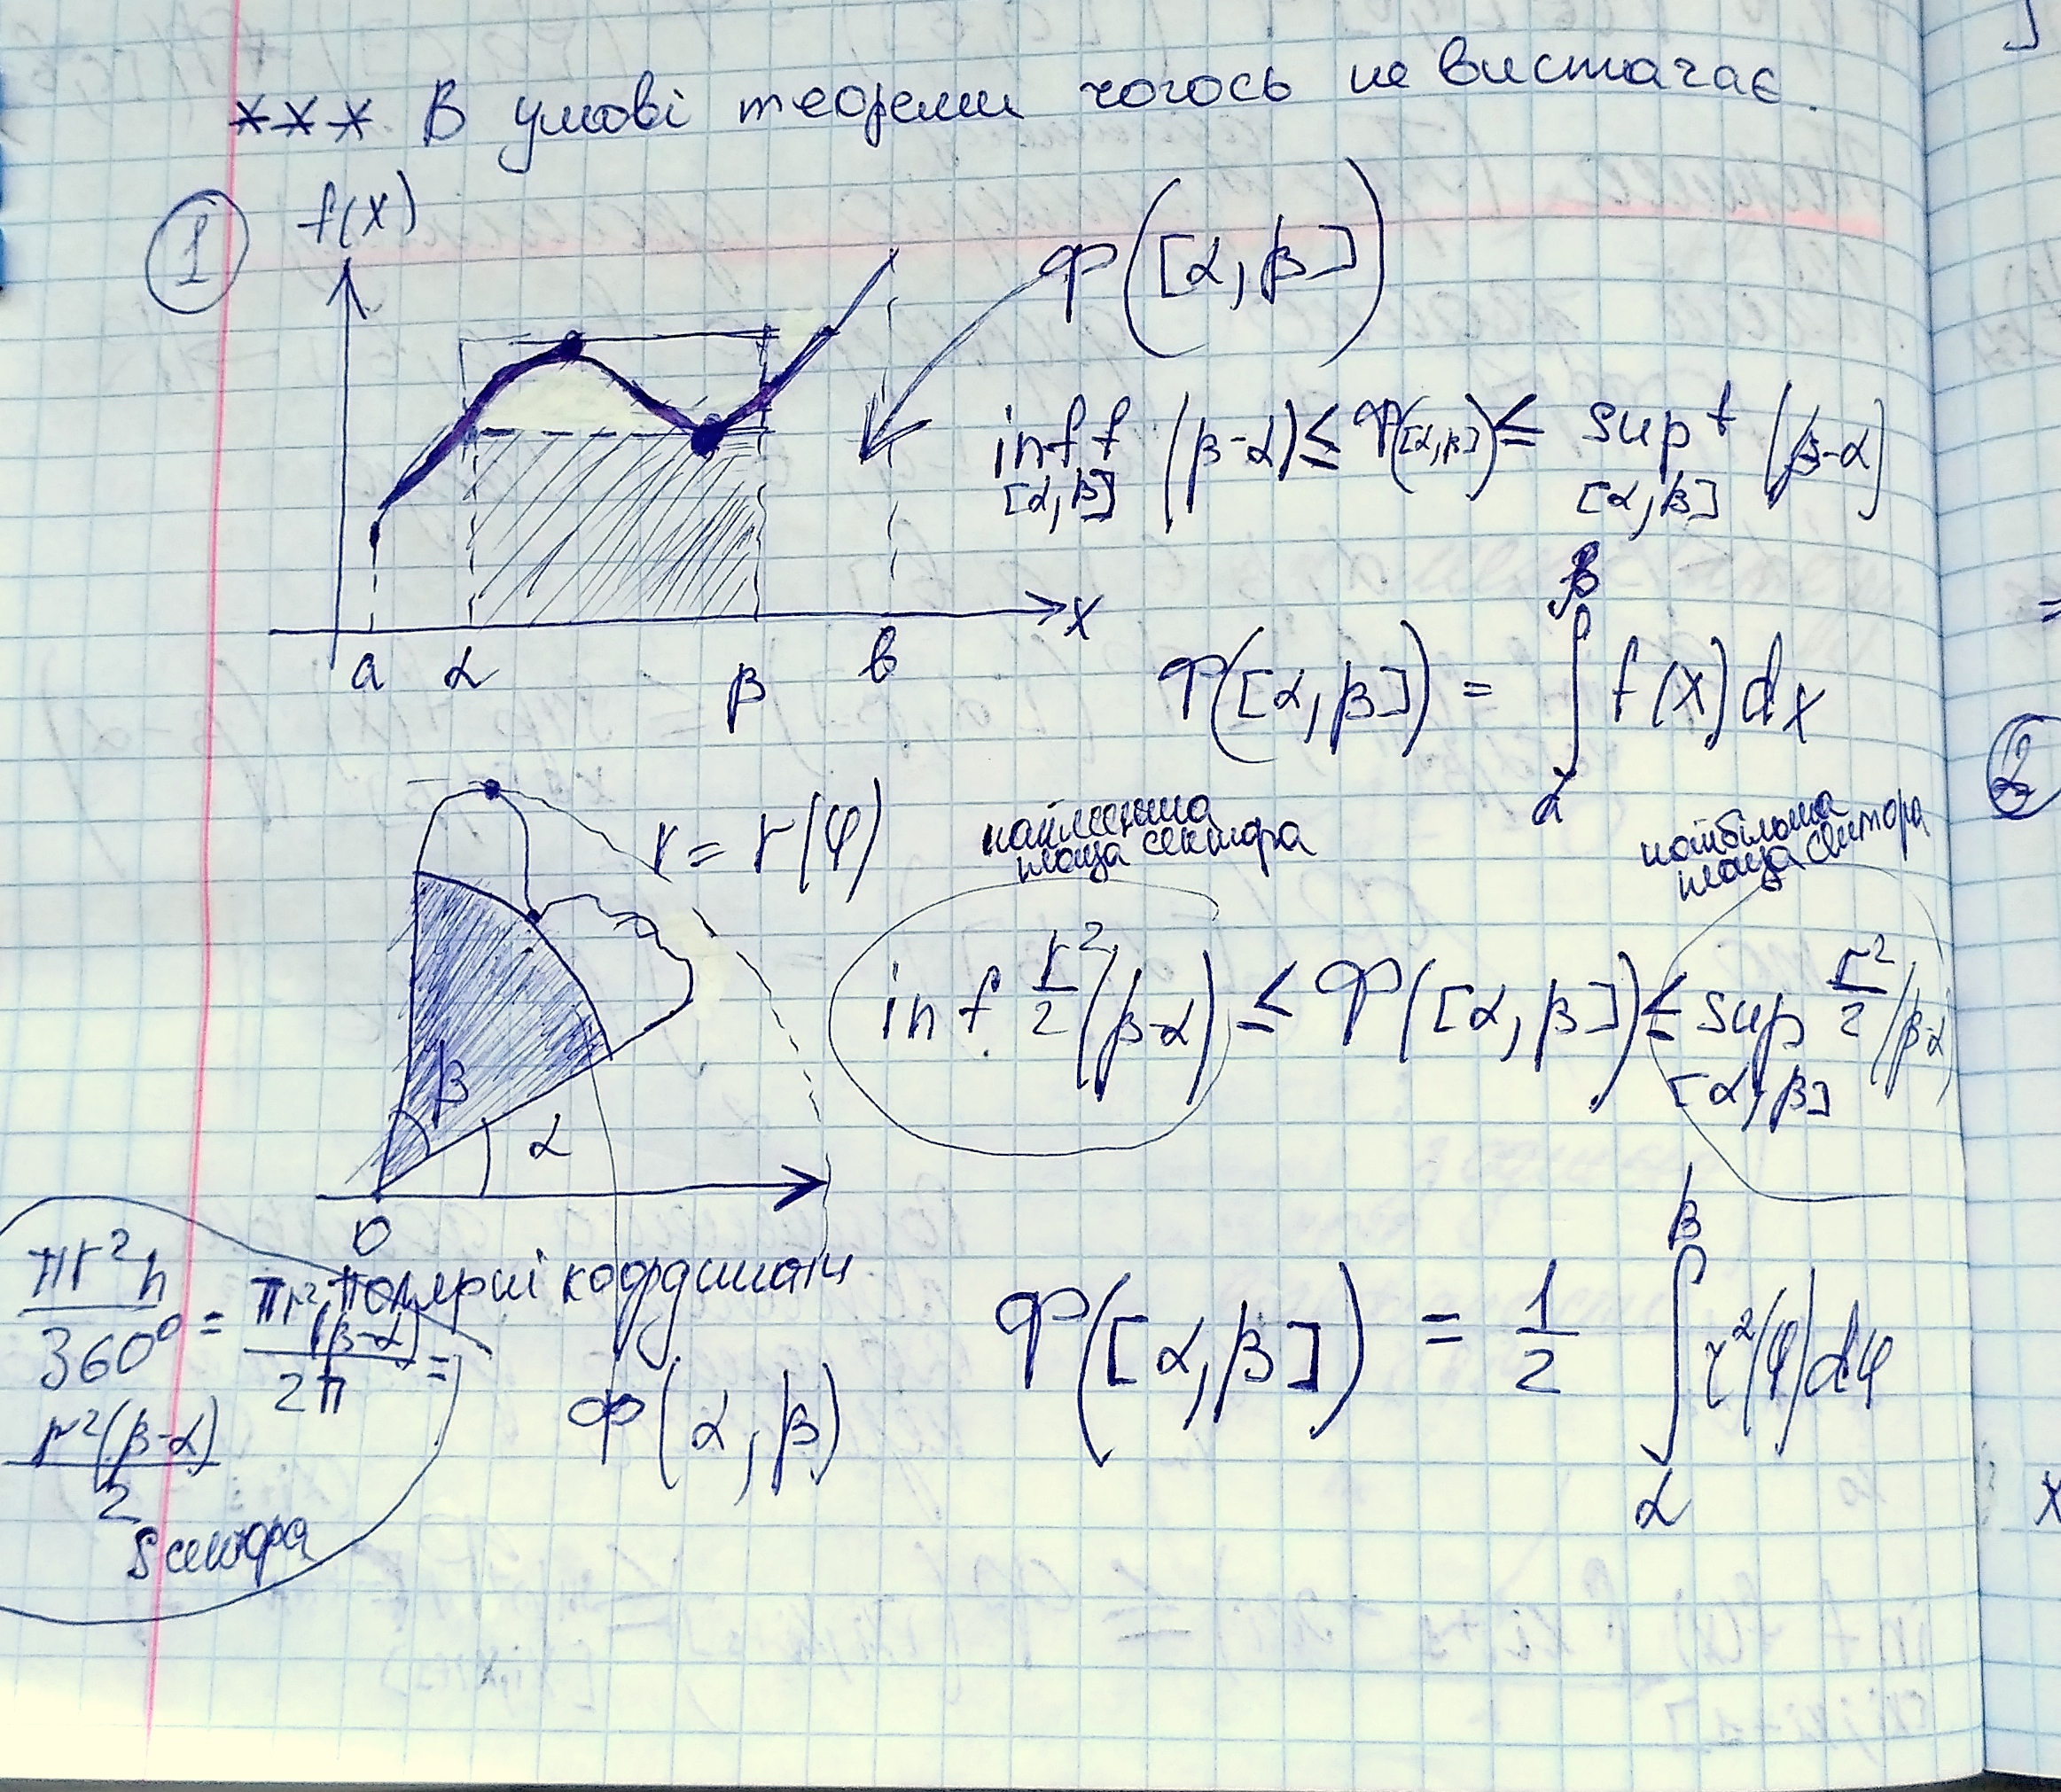
\includegraphics[scale = 0.2]{image1.jpg}
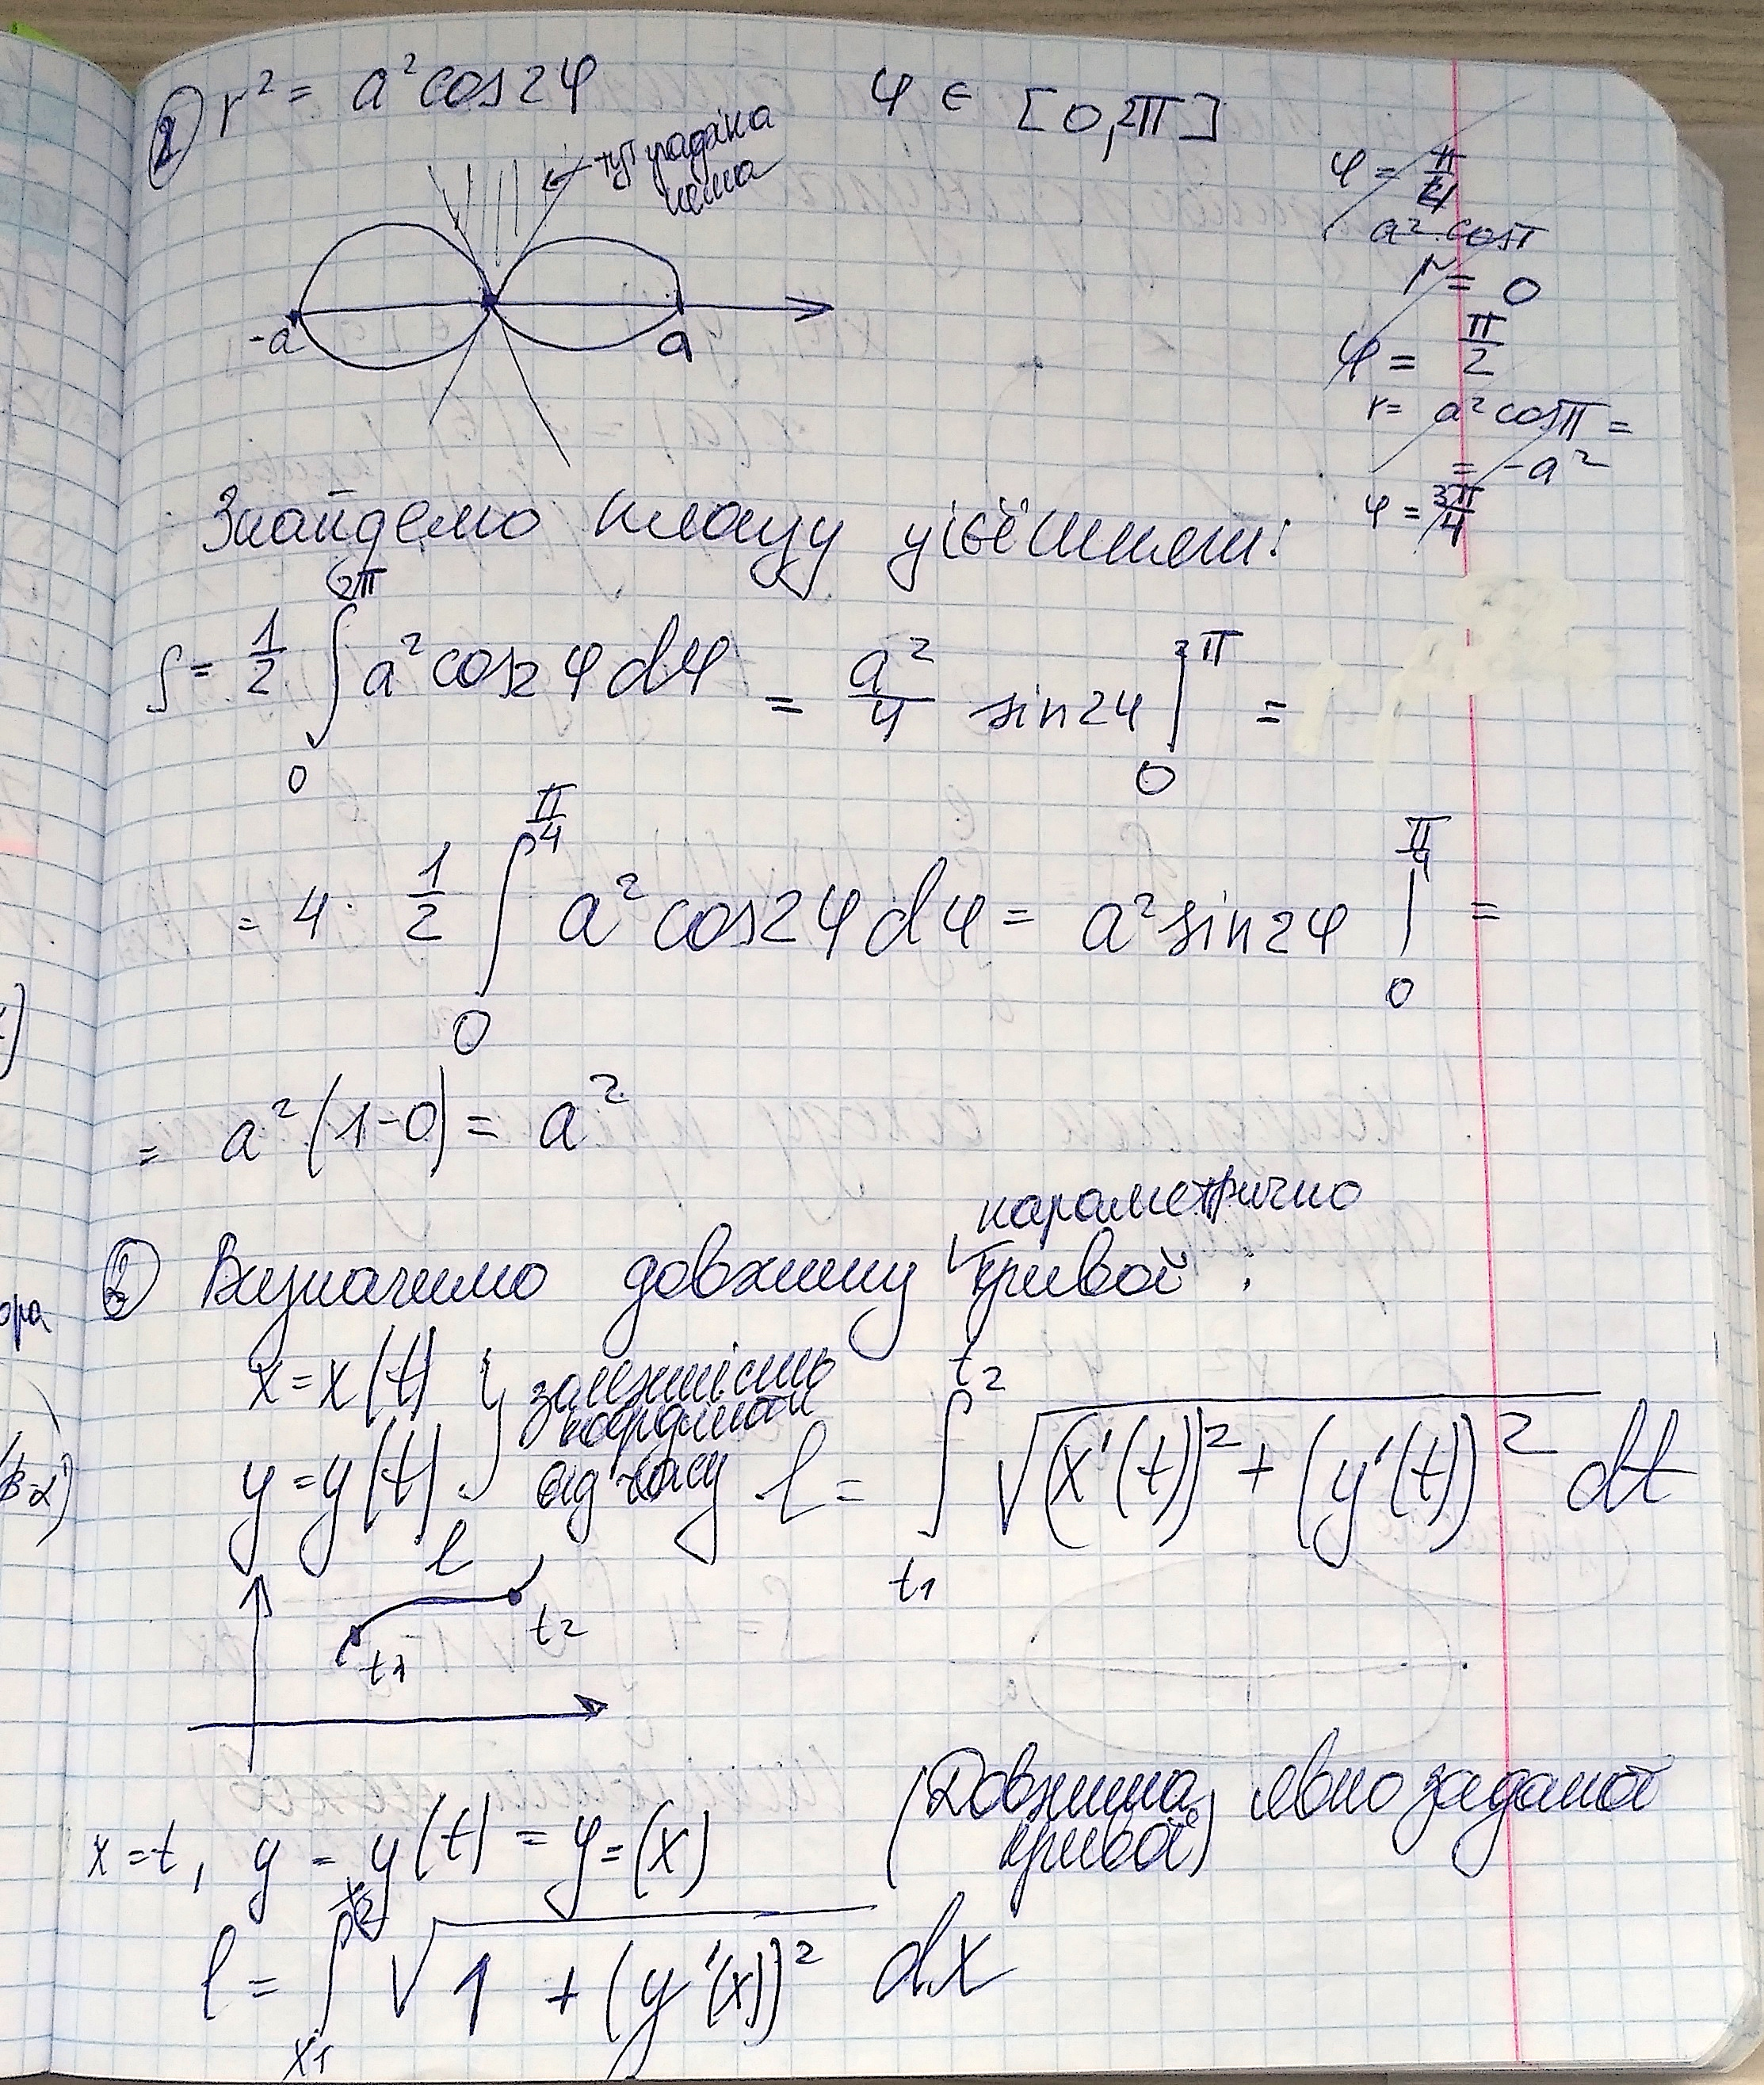
\includegraphics[scale = 0.2]{image2.jpg}
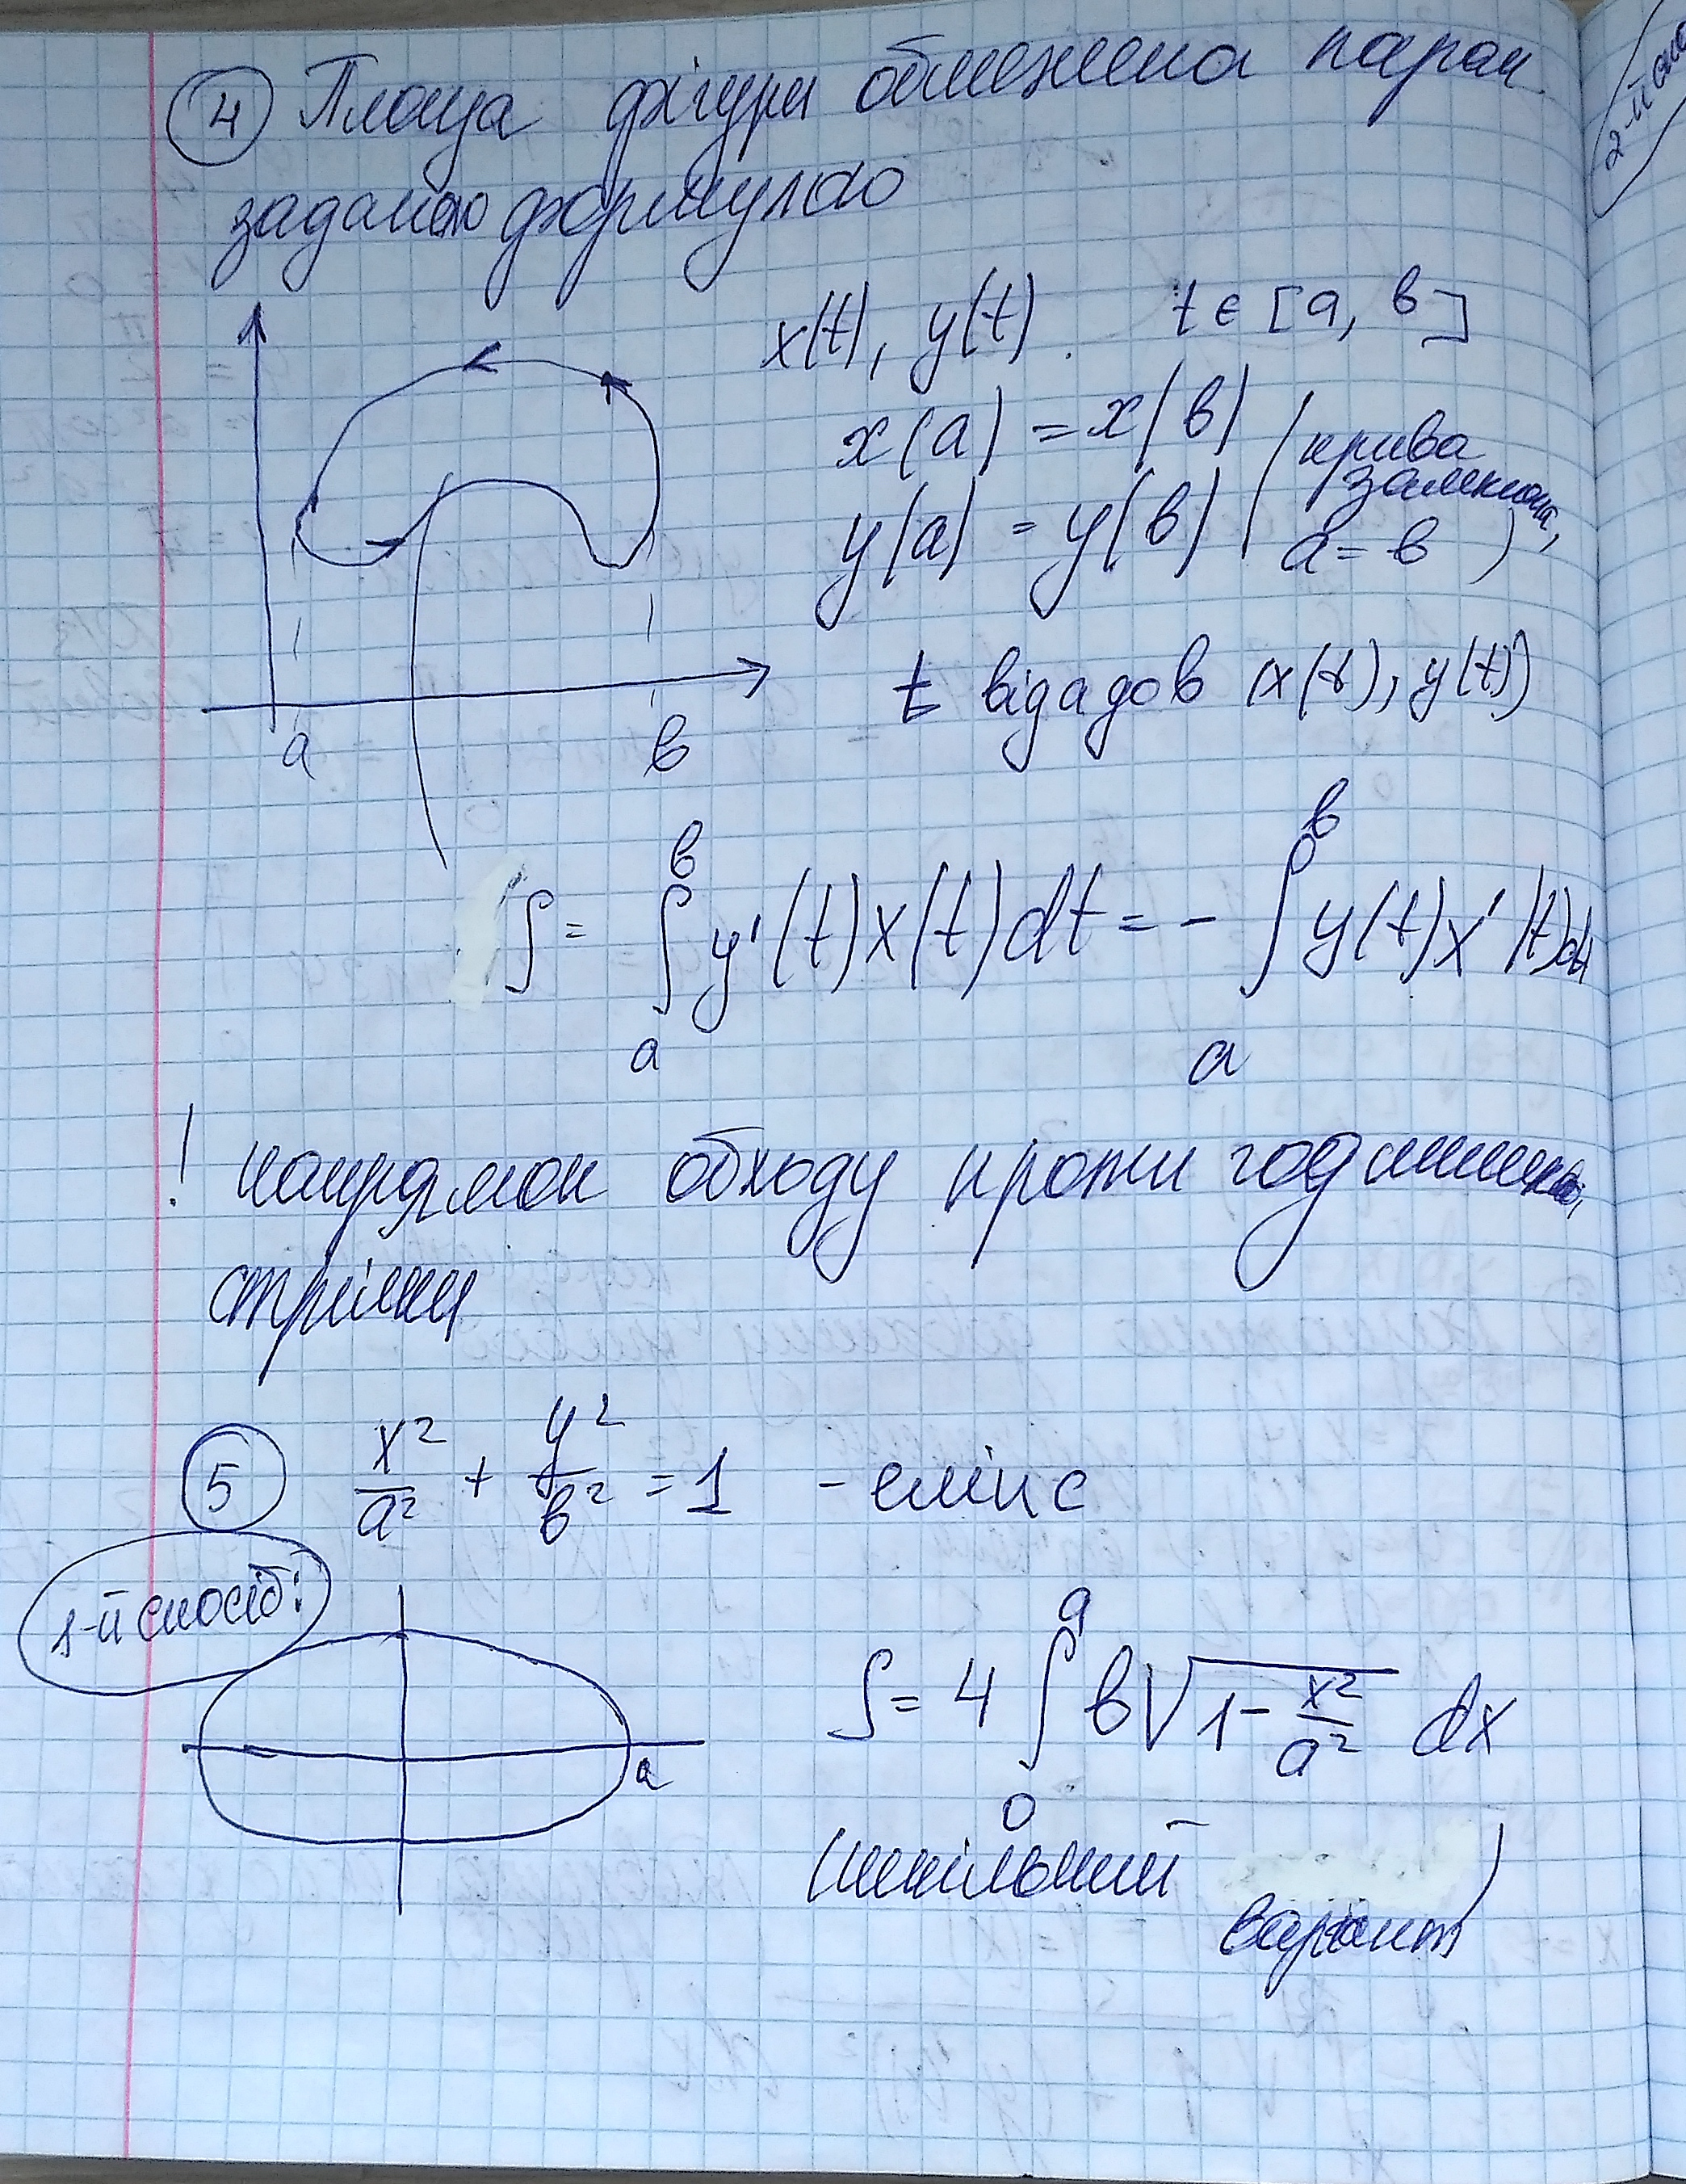
\includegraphics[scale = 0.2]{image3.jpg}
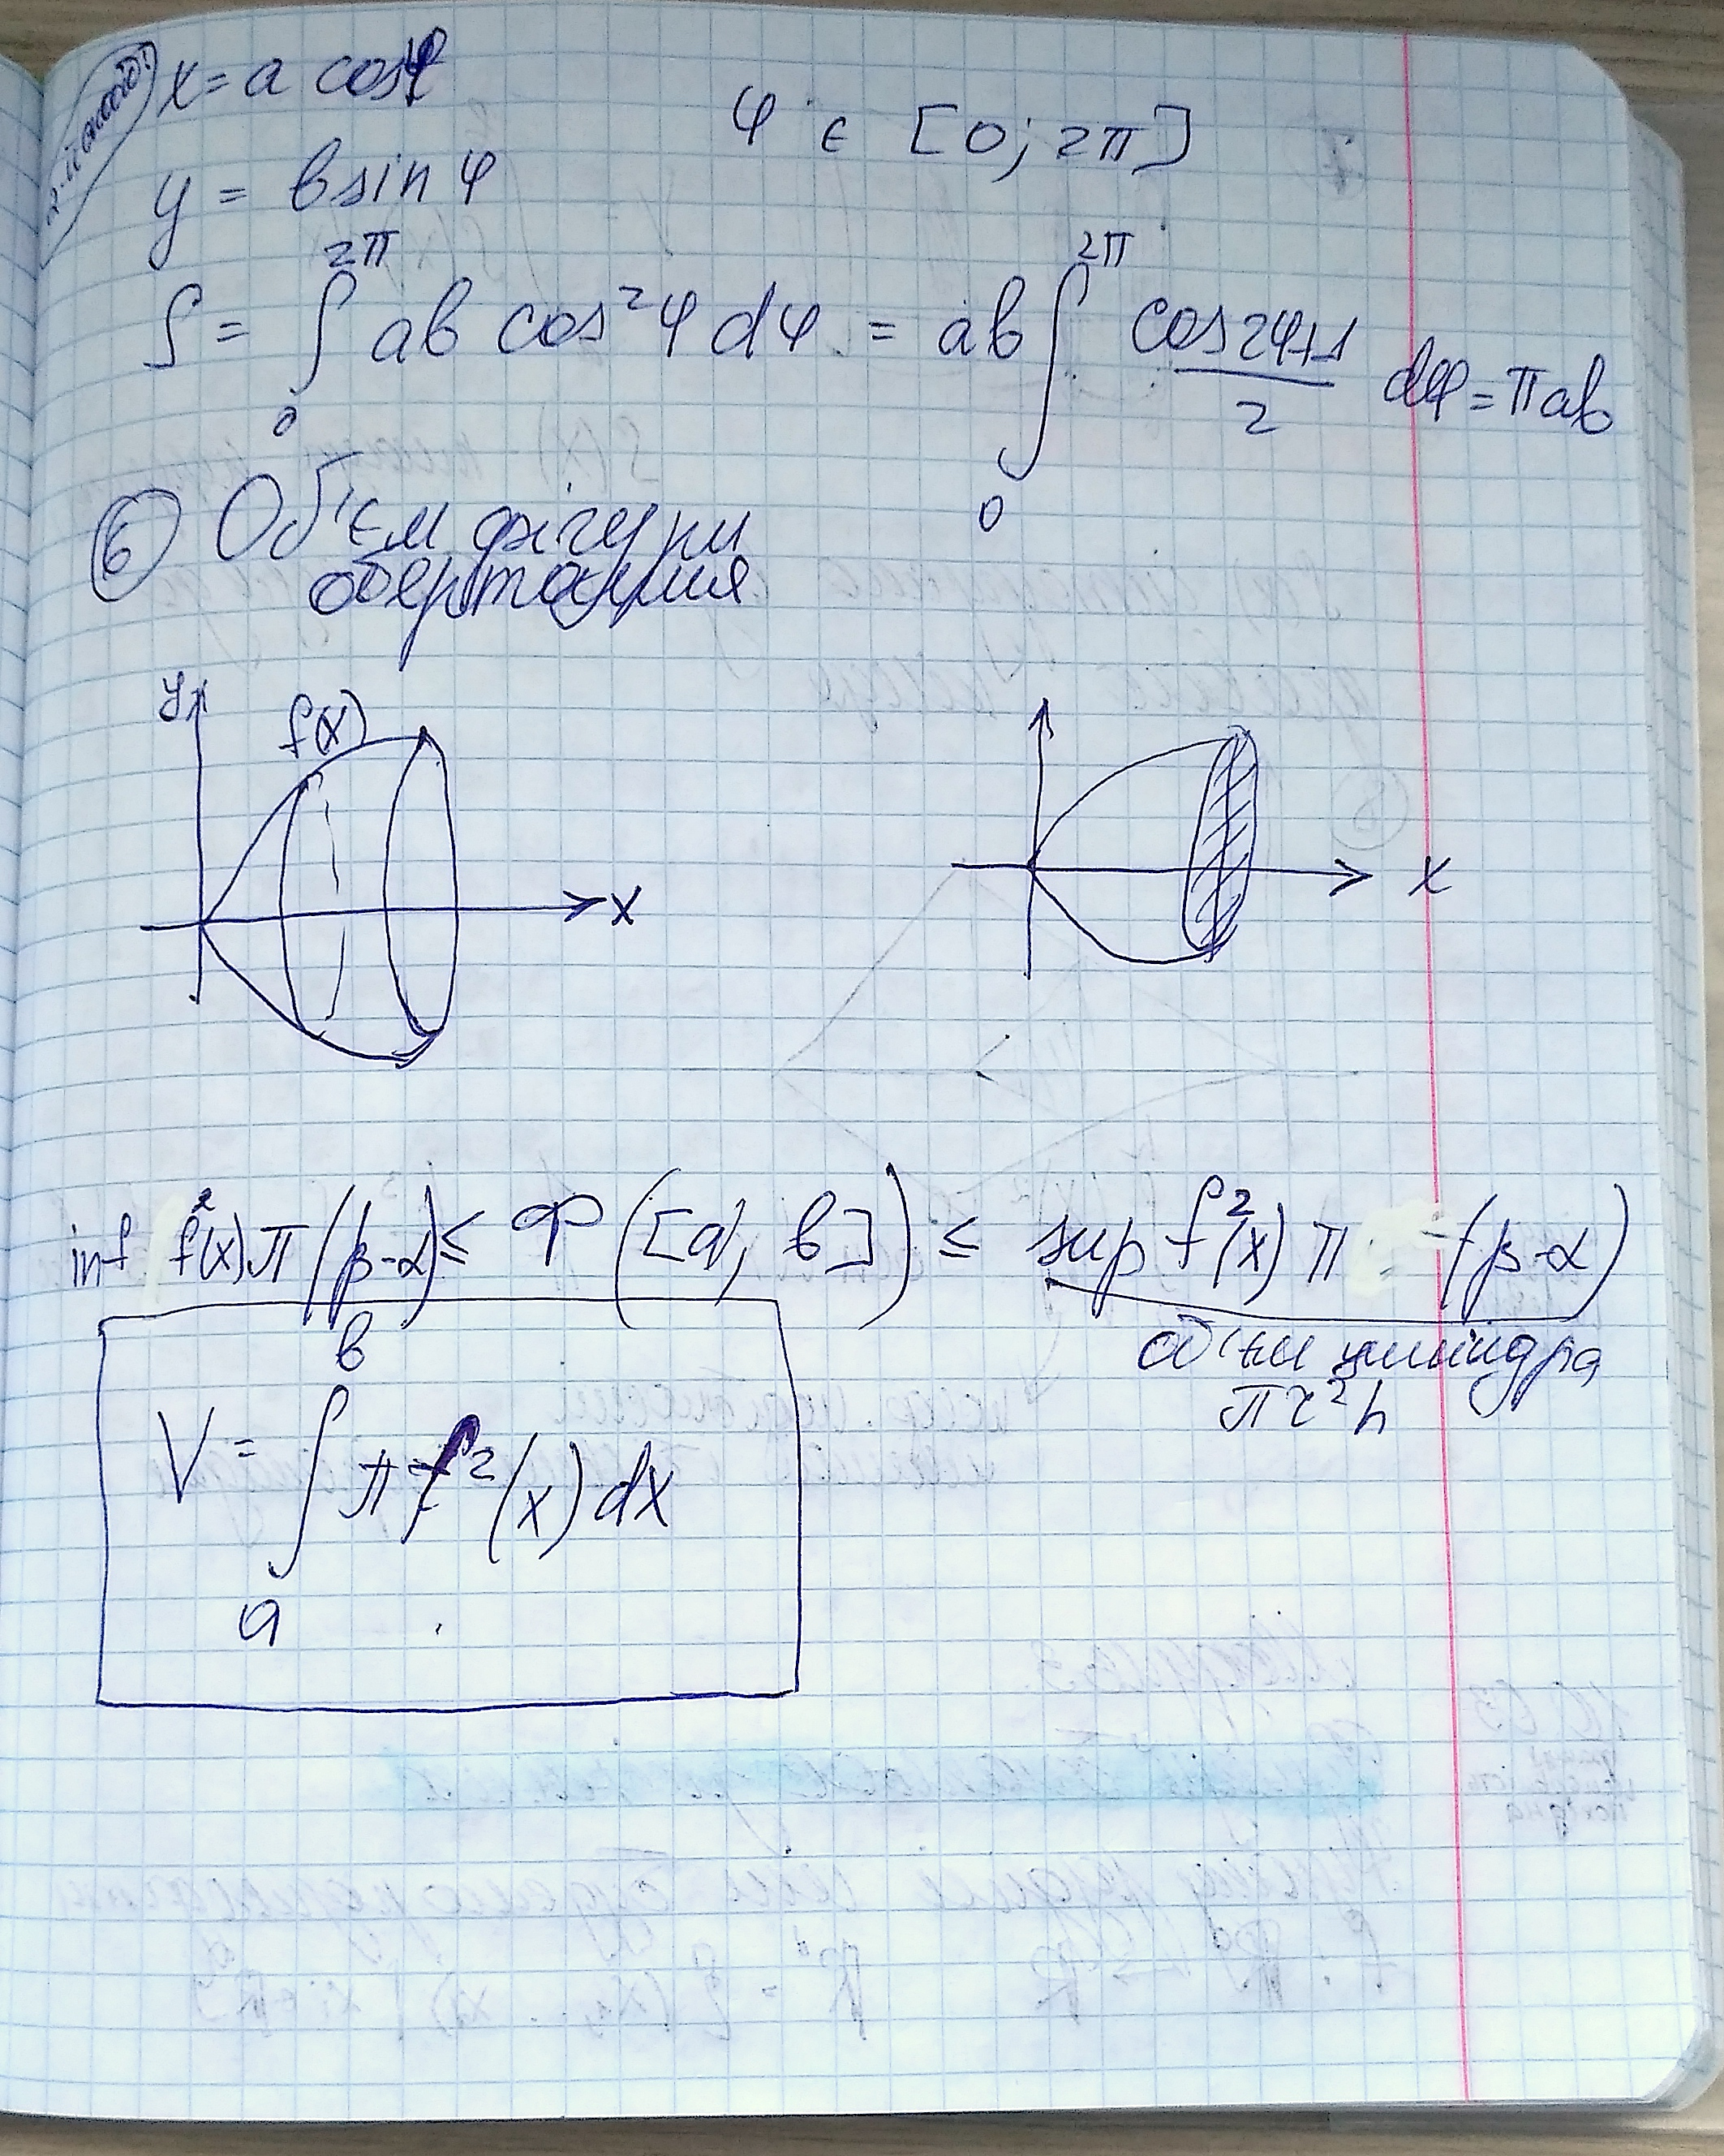
\includegraphics[scale = 0.2]{image4.jpg}
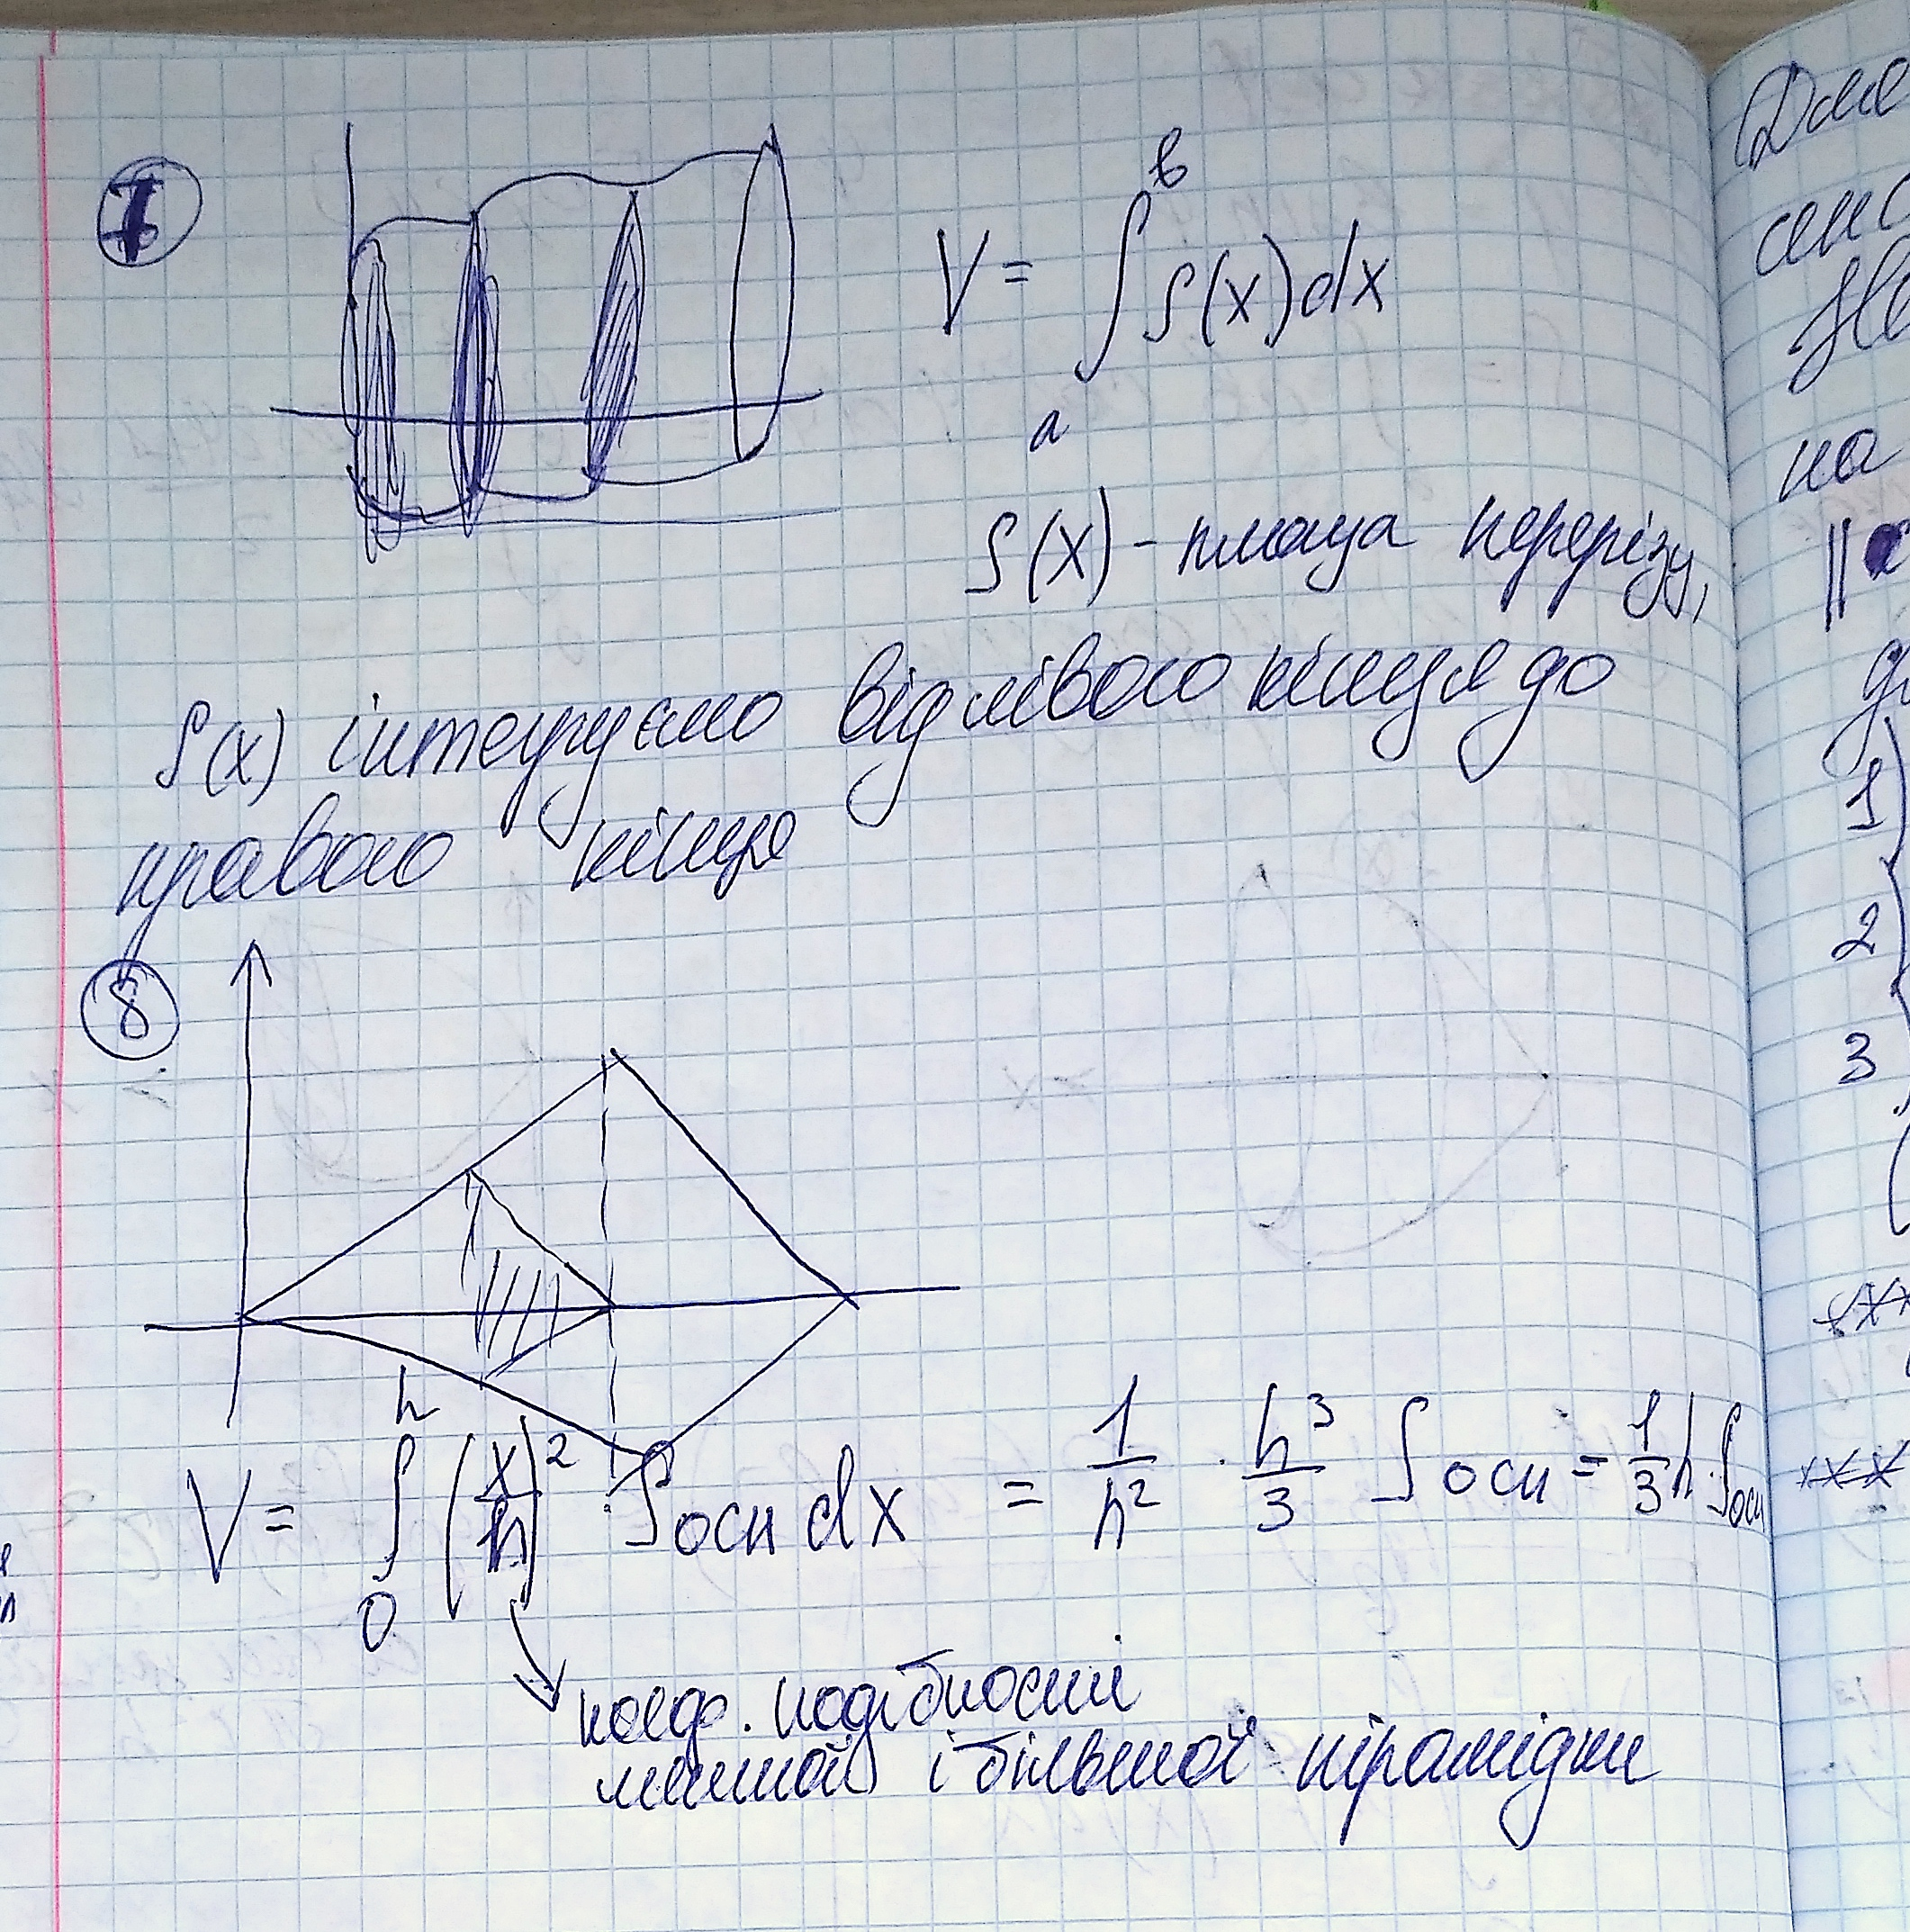
\includegraphics[scale = 0.2]{image5.jpg}
=======
\vspace{5 mm}

Нехай $P$ --- розбиття. $P_1 = P \cup \{ x^{*}\}$.

$$\overline S_p(f) = \sum_{k = 1}^m M_{k} \Delta x_k + M_{m+1}\Delta x_{m+1} + \sum_{k = m+2}^n M_k \Delta x_k$$

$$\overline S_{p_1}(f) = \sum_{k = 1}^m M_{k} \Delta x_k + \sup_{x \in [x_{m}; x^{*}]} f(x) (x^* - x_m) + \sup_{x \in [x^{*}; x_{m+1}]} f(x) (x_{m+1} - x^*) + \sum_{k = m+2}^n M_k \Delta x_k$$
$$A \subset B \Longrightarrow \sup_{A} f \leq \sup_{B} f$$
$$\sup_{x \in [x_{m}; x^{*}]} f(x) \leq M_{m+1}$$
$$\sup_{x \in [x^{*}; x_{m+1}]} f(x) \leq M_{m+1}$$
>>>>>>> 5f31d61c42ed2880ed77edce41b66cab0eaf8166

$$\overline S_{p_1}(f) \leq \sum_{k = 1}^m M_{k} \Delta x_k + M_{m+1}\Delta x_{m+1} + \sum_{k = m+2}^n M_k \Delta x_k$$
$$\overline S_p \geq \overline S_{p+1}$$
Додаючи точку до розбиття, верхня (з супремами) інтегральна сума може зменшитися або залишитис такою ж.

<<<<<<< HEAD
\end{document}  
=======
Тому зрозуміло, що 
$$P_1 \subset P_2 \Longrightarrow \overline S_{p_1} \geq \overline S_{p_k}, \underline S_{p_1} \leq \underline S_{p_2}$$
>>>>>>> 5f31d61c42ed2880ed77edce41b66cab0eaf8166

\textbf{Наслідок:}

$$\forall P_1, P_2 \overline S_{P_1}(f) \geq \underline S_{P_2}(f)$$ 

Розглянемо розбиття $P = P_1 \cup P_2$.
$$\overline S_{P_1} \geq \overline S_{p} \textrm{(з попередньої теореми $P_1 \subset P_2 \Longrightarrow \overline S_{P_1} \geq \overline S_{p}$)}$$
$$\underline S_{P} \geq \underline S_{P_2}$$
$$\overline S_{P_1} \geq \overline S_{P} \geq \underline S_{P} \geq \underline S_{P_2}$$
$$\overline S_{P_1} \geq \underline S_{P_2}$$
Що й треба було довести.

\vspace{3mm}

Розглянемо всі можливі верхні суми. $\overline S_{P} (f)$. Ця множина є обмеженою знизу (Необхідна умова інтегрованості за Ріманом). 
Тому існує $\inf_{P} \overline S_{P} (f) = \overline \int f dx$. Назвемо це число верхнім інтегралом Дербу. Аналогічно 
нижній інтеграл Дербу $\underline \int f dx = \sup_{P} \underline S_{p} (f)$.

\vspace{3mm}

Розглянемо нерівність $\overline S_{P_1} (f) \geq S_{P_2} (f)$. 
Зафіксуємо $P_2$. Тоді 
$$\forall P_1 \overline S_{P_1} (f) \geq \underline S_{P_2} \Longrightarrow \inf \overline S_{P_1} (f) \geq \underline S_{P_2} (f)$$
(Всі елементи множини $>$ за фіксоване число $\Longrightarrow$ $>$ за інфінум.)

Аналогічно для $P_2$ та супремума:

Зафіксуємо $P_1$. Тоді:
$$\forall P_2 \ \underline S_{P_2} (f) \leq \overline S_{P_1} (f) \Longrightarrow \sup \overline S_{P_1} (f) \leq \underline S_{P_1} (f)$$
Звідcи $\overline \int fdx \geq \underline f dx$.

\textbf{Означення}. Функція $f$ називається інтегровною за Дарбу, якщо $\overline \int f dx = \underline \int fdx$. (Найкраше наближення зверху = найкраще наближення знизу).

\textbf{Теорема. (Критерій інтегрованості за Дарбу)}. Функція $f$ є інтегровною за Дарбу тоді й тільки тоді, коли:
$$\forall \varepsilon > 0 \ \exists P : |\overline S_{p}(f) - \underline S_{P} (f)| < \varepsilon$$
(Можна підібрати число, для якого верхня і нижня інтегральні суми відрізняються на мале число)

\textbf{Доведення}

\begin{itemize}
\item $\Longleftarrow.$
$$\underline S_{P} (f) fdx \leq \overline \int fdx \leq \overline S_{P} (f)$$ 
$$\underline S_{P} (f) \leq \underline \int fdx \leq \overline \int f dx \leq \overline S_{P} (f)$$
$$\varepsilon \geq \overline S_{P} (f) - \underline S_{P} (f) \geq \overline \int f dx - \underline \int f dx \geq 0$$

Отже, $\overline \int f dx - \underline f dx = 0$.

\item $\Longrightarrow.$

Зафіксуємо $\varepsilon > 0$. Тоді супремум $\inf \overline S_{P} (f) = \overline \int f dx$ є точкою дотику 
в будь-якому $\varepsilon$-околі множини.
$$\exists P_{1} \ \overline \int f dx \leq \overline S_{P_1} (f) \leq \overline \int fdx + \frac{\varepsilon}{2}$$
$$\exists P_{2} \ \underline \int f dx \leq \underline S_{P_2} (f) \leq \underline \int fdx $$

Розглянемо $P = P_1 \cup P_2$. Збільшуємо розбиття, збільшуємо точність, верхня інтегральна сума збільнується (або залишається такою ж).

$$0 \leq \overline S_{P} (f) - \underline S_{P} (f) \leq \overline S_{P_1} - \underline S_{P_2} (f) < \varepsilon$$
Що і треба було довести.
\end{itemize}

\vspace{5mm}

\textbf{Теорема.} Функція $f$ є інтегрованою за Дарбу тоді й тільки тоді, коли $f$ інтегровна за Ріманом і їх інтеграли співпадають.

\vspace{3mm}

\textit{Приклад 1.}
$$0 = x_0,\ x_k = \frac{1}{n},\ x_n = 1$$
$$\overline S_{P} (f) = \sum_{k=1}^n M_k \cdot \Delta x_k = \sum_{k=1}^n \frac{k}{n} \cdot \frac{1}{n}$$
$$M_k = \sup_{[x_{k-1}, x_k]} x = x_k = \frac{k}{n}$$
$$\underline S_{P} (f) = \sum_{k = 1}^n M_k \Delta x_k = \sum_{k=1}^n x_k + \Delta x_k = \sum_{k=1}^{n} \frac{k-1}{n} \cdot \frac{1}{n}$$
$$\overline S_{P}(f) - \underline S_{P} (f) = \frac{1}{n}$$
$\frac{1}{n}$ може бути як завгодно мале, а тому $x \in R([0,1])$ (інтегрована за Ріманом).
\vspace{3mm}

\textit{Приклад 2.}
$$D(x) =  \begin{cases} 1 &, x \in \mathbb{Q} \\
						  0 &, x \in \mathbb{R} \setminus \mathbb{Q} \end{cases}$$
Функцію розглядаємо на проміжку $[0,1]$.

$$\overline S_{P} (D) = \sum_{k=1}^n \sup_{x \in [\ldots]} D(x) = \sum_{k=1}^n \Delta x_k = 1$$
$$\underline S_{P} (D) = \sum_{k=1}^n( \inf_{x \in [\ldots]} (D(x)) \cdot  \Delta x_k) = 0$$
$$\forall p : \overline S_{p}(D) - \underline S_{p} (D) > \frac{1}{13} =  \varepsilon$$
Отже, $D \notin R([0,1])$.

\begin{center}
	\textbf{\LargeМножини Лебегової міри нуля} 
\end{center}

\textbf{Означення} Множина $A \subset \mathbb{R}$ має міру нуль, якщо $\forall \varepsilon > 0 \ \exists$ не більш як зліченна кількість $ (\alpha_1,\beta_1), (\alpha_2,\beta_2), \ldots$ такі, що:

\begin{enumerate}

\item $A \subset \bigcup_{k=1}^{\infty} (\alpha_k, \beta_k)$ (Множину можна покрити інтервалами, що є завгодно малими)

\item $\sum (\beta_k - \alpha_k) < \varepsilon$

\end{enumerate}

\textit{Приклад}:

\begin{enumerate}

\item $A = \{ x_0\}$
\item $A = \{ x_1, x_2, \ldots, x_n\}$
\item $A = (0; \frac{1}{2})$ При $\varepsilon < \frac{1}{2}$ покритий не існує. (Якщо є неперервна множина, з більше, ніж однієї точки), $A$ не має точки нуль).
\item $A = \{ x_1, x_2, \ldots\}$
\end{enumerate}

\textbf{Властивості:}

\begin{enumerate}

\item Якщо $A$ -- зліченна, або обмежена, то $A$ має міру нуль.
\item Якщо $\exists \alpha, \beta : (\alpha, \beta) \subset A \Longrightarrow A$ не має міру нуль.
\item Незліченні (континуальні) множини теж мають міру нуль.
\item Якщо $A_1, A_2, \ldots$ мають міру нуль, то їх об'єднання теж має міру нуль.  

\end{enumerate}

\textbf{Приклад:}

\begin{itemize}

\item $Q \cap [0,1]$ -- зліченна, тож має міру нуль.
\item $(\mathbb{R} \setminus \mathbb{Q}) \cap [0,1]$. Якщо припустити, що $(\mathbb{R} \setminus \mathbb{Q}) \cap [0,1]$ 
має міру нуль, то за властивістю $4$:

$(\mathbb{Q}\cap[0,1]) \cup (\mathbb{R} \setminus \mathbb{Q}) \cap [0,1] = [0,1]$ теж має міру 0. Але це суперечить властивості $2$.

\end{itemize}
 

\textbf{Критерій Лебега інтегровності за Ріманом}

Нехай $f$ -- обмежена на $[a,b]$. Тоді $f \in R([a,b])$ тоді й тільки тоді, коли множина точок розриву функції $f$ на $[a,b]$ має міру $0$.
(Тобто коли точок розриву не більше, ніж зліченна кількість).

\textbf{Приклади:}

\begin{enumerate}
\item D(x) = $\begin{cases} 1 &, x \in \mathbb{Q} \\ 0 &, x \notin \mathbb{Q} \end{cases}$ на проміжку $[0,1]$.

$E_{D} = [0,1]$ -- не має міру $0$ за властивостю $2$.

Отже, за критерієм $D \notin R([0,1])$.

\item $f(x) = \frac{x - \frac{1}{2}}{|x - \frac{1}{2}|} = \begin{cases} 1 &, x > \frac{1}{2} \\ -1 &, x < \frac{1}{2} \end{cases}$

$E_f = \{\frac{1}{2}\}$ -- множина точок розриву має міру нуль. Отже, $f(x) \in R([0,1])$.

\item Функція Рімана:

$$f(x) = \begin{cases} 0 &, x \in \mathbb{R} \setminus \mathbb{Q} \\ 
					   \frac{1}{n} &, x = \frac{m}{n}, \textrm{НСД($m$,$n$) = 1}
		 \end{cases}$$
$E_f = \mathbb{Q} \cap [0,1]$. Отже, $f$ інтегрована.

\item $f(x) = \ln x$

$E_f = \{0\}$ -- точки розриву. Але $f(x)$ необмежена, тому не є інтегрованою за Ріманом на $[0,1]$.

\end{enumerate}
 
\end{document}  